\documentclass[a4paper,13pt]{report}
\usepackage{tikz}
\usepackage[authoryear]{natbib}
\usetikzlibrary{calc}
\usepackage{placeins}
\usetikzlibrary{shapes.geometric, arrows.meta, positioning}
\usepackage{geometry}
\usepackage{float}
\usepackage{times}
\usepackage{graphicx}
\usepackage{booktabs}
\usepackage{enumitem}
\usepackage{fancyhdr}
\usepackage{tocloft}
\usepackage{hyperref}
\usepackage{caption}
\bibliographystyle{apa}
\usepackage{setspace}


% Set margins
\geometry{left=3cm, right=2cm, top=2cm, bottom=2cm}

% Page number at top center
\pagestyle{fancy}
\fancyhf{}
\fancyhead[C]{\thepage}
\renewcommand{\headrulewidth}{0pt}

% Line spacing
\onehalfspacing

% Table of contents formatting
\renewcommand{\cftchapleader}{\cftdotfill{\cftdotsep}}
\renewcommand{\cftsecleader}{\cftdotfill{\cftdotsep}}

\begin{document}

% Cover page (Form 01)
\begin{titlepage}
  \centering
  
  % Thêm khung viền với TikZ
  \begin{tikzpicture}[remember picture, overlay]
    % Định nghĩa kích thước khung viền
    \def\borderwidth{0.5pt} % Độ dày viền
    \def\borderdistance{1.5cm} % Khoảng cách từ viền đến lề trang
    
    % Tọa độ các góc của khung viền
    \coordinate (top-left) at ([shift={(\borderdistance,-\borderdistance)}]current page.north west);
    \coordinate (top-right) at ([shift={(-\borderdistance,-\borderdistance)}]current page.north east);
    \coordinate (bottom-left) at ([shift={(\borderdistance,\borderdistance)}]current page.south west);
    \coordinate (bottom-right) at ([shift={(-\borderdistance,\borderdistance)}]current page.south east);
    
    % Vẽ khung viền
    \draw[line width=\borderwidth] (top-left) -- (top-right) -- (bottom-right) -- (bottom-left) -- cycle;
    
    % Thêm họa tiết ở các góc
    \def\cornerdeco{ % Định nghĩa họa tiết góc
      \draw[decoration={coil, amplitude=2pt, segment length=4pt}, decorate, line width=\borderwidth]
      (0,0) -- (0.5cm,0) arc (0:90:0.5cm) -- (0,0.5cm);
    }
    
  \end{tikzpicture}

  \vspace*{1cm} % Khoảng cách từ đầu trang
  \centering
  \vspace*{1cm}
  {\Large \textbf{VIETNAM NATIONAL UNIVERSITY, HANOI}} \\
  \vspace{0.5cm}
  {\Large \textbf{INTERNATIONAL SCHOOL}} \\
  \vspace{1cm}
  \includegraphics[width=0.3\textwidth]{logo.png} \\
  \vspace{1cm}
  {\Large \textbf{STUDENT RESEARCH REPORT}} \\
  \vspace{1cm}
  {\Huge \textbf{Cross-platform Emotion Recognition for \\ Users using YOLOv12 Object Detection}} \\
  \vspace{0.5cm}
  {\Large CN.NC.SV.24.20} \\
  \vspace{2cm}
  {\Large \textbf{Team Leader: Phan Nam Khanh}} \\
  {\Large ID: 22070980} \\
  {\Large Class: ICE2022A} \\
    \vspace{5cm}
  {\Large Hanoi, 2025}
\end{titlepage}

%---------------------------------------------COVER--------------------------------------------------
\clearpage
\chapter*{ACKNOWLEDGEMENTS}
\addcontentsline{toc}{chapter}{ACKNOWLEDGE}
% Reset chapter counter to 0 and adjust section numbering to remove chapter prefix
\setcounter{chapter}{0}
\renewcommand{\thesection}{\arabic{section}}
%viet liter-------------------------------------------------------------- 
We would like to express our sincere gratitude and appreciation to the individuals and organizations who have contributed to the completion of this research report titled "Cross-platform Emotion Recognition for Users using YOLOv12 Object Detection."

First of all, we would like to express our heartfelt thanks to PhD. Kim Dinh Thai for his invaluable guidance, support, and expertise throughout the research process. His insightful feedback and advice helped shape the direction of this research report.
We truly feel honored to have had the opportunity to work with such a talented and dedicated mentor. We hope to continue collaborating with him in the future and to learn even more from his extensive knowledge and experience.

We would also like to thank the participants whose support and cooperation provided valuable insights and data for this study. Your willingness to share your knowledge and experiences has greatly contributed to the accuracy and reliability of our research.

In addition, we would like to express our appreciation to the teachers at VNU - IS for creating a supportive learning environment and equipping us with useful knowledge throughout our academic journey.

Thanks again to everyone who contributed to this research report. Your support has been indispensable, and we are truly grateful for your participation in this effort.

Best regards,



\clearpage
\chapter*{TEAM LEADER INFORMATION}
\addcontentsline{toc}{chapter}{TEAM LEADER INFORMATION}
% Reset chapter counter to 0 and adjust section numbering to remove chapter prefix
\setcounter{chapter}{0}
\renewcommand{\thesection}{\arabic{section}}
\section{Student Profile}
\begin{itemize}
  \item \textbf{Full Name:} Phan Nam Khanh
  \item \textbf{Date of Birth:} October 21, 2004
  \item \textbf{Place of Birth:} Hanoi, Vietnam
  \item \textbf{Class:} ICE2022A
  \item \textbf{Program:} Informatics and Computer Engineering
  \item \textbf{Address:} Ba Dinh, Hanoi
  \item \textbf{Phone/Email:} (+84)852232174 / 22070980@vnu.edu.vn
\end{itemize}

\begin{minipage}[t]{0.3\textwidth}
    \vspace*{-7cm} % Move the image up to the top of the page (adjust as needed)
    \hspace*{11cm} % Push the image to the right
    \includegraphics[width=0.8\textwidth]{Ảnh thẻ.jpg} % Adjust the image filename as needed
\end{minipage}

\section{Academic Results}
\begin{table}[h]
  \centering
  \caption{Academic Results}
  \label{tab:academic}
  \begin{tabular}{lcc}
    \toprule
    Academic Year & Overall Score & Academic Rating \\
    \midrule
     &  &  \\
     &  &  \\
    \bottomrule
  \end{tabular}
\end{table}



\section{Other Achievements}
\begin{itemize}
   
\end{itemize}


\end{flushright}

\begin{flushleft}
    \vspace{2cm}
    \textbf{Advisor} \hfill \textbf{Hanoi, 2025} \\
    (Sign and write full name) \hfill \textbf{Team Leader} \\

    \begin{minipage}{0.2\textwidth}
        \centering
        \includegraphics[width=1.3\textwidth,height=1.3\textheight,keepaspectratio]{teacher sign.png} \\
        \vspace{3pt}
        \small Kim Dinh Thai
    \end{minipage}
    \hfill
    \begin{minipage}{0.3\textwidth}
        \centering
        \includegraphics[width=1\textwidth,height=1\textheight,keepaspectratio]{leader sign.png} \\ 
        \vspace{3pt}
        \small Phan Nam Khanh
    \end{minipage}
     \\
\end{flushleft}



% Table of Contents
\clearpage
\tableofcontents
\addcontentsline{toc}{chapter}{TABLE OF CONTENTS}

% List of Tables
\clearpage
\listoftables
\addcontentsline{toc}{chapter}{LIST OF TABLES}

% List of Figures
\clearpage
\listoffigures
\addcontentsline{toc}{chapter}{LIST OF FIGURES}

% Chapter: Introduction
\clearpage
\chapter{INTRODUCTION}
\section{Project Name}
\textbf{Cross-platform Emotion Recognition for Users using YOLOv12 Object Detection}

\section{Project Code}
CN.NC.SV.24\textunderscore20



\section{Member List}
\begin{table}[h]
  \centering
  \caption{Team Members}
  \label{tab:members}
  \begin{tabular}{lcc}
    \toprule
    Full Name & Class & ID \\
    \midrule
    Phan Nam Khanh & ICE2022A & 22070980 \\
    Nguyen Van Giang & FDB2022B & 22070278 \\
    Nguyen Thanh Lan & ICE2022B & 22071014 \\
    Nguyen Anh My & ICE2022B & 22071007 \\
    \bottomrule
  \end{tabular}
\end{table}

\section{Advisor(s)}
Kim Dinh Thai, Faculty of Engineering and Technology, Ph.D.

\section{Abstract}
This study proposes an emotion recognition system based on computer vision and artificial intelligence chatbot using YOLOv12 and API by gemini 1.5 flash pro, utilizing facial analysis to develop an emotional assistant capable of natural interaction with users. The dataset comprises 8,821 images across eight basic emotion classes include anger, happy, neutral, sad, contempt, surprised, fear, disgust , collected from various sources, meticulously processed, labeled with bounding boxes, and augmented using techniques such as brightness adjustment, blurring, rotation, and more. The model was trained in Google Colab using a Tesla T4 GPU and Kaggle using GPU P100, employing YOLOv12 and CNN architectures optimized for high performance and precision. The results demonstrate exceptional accuracy, with an mAP@0.5 score exceeding 94.1\% and mAP@0.5:0.95 score exceeding 85.1\% in the test set. The system operates efficiently in real-time on web platforms and some functions on the Android application "EVision," leveraging TensorFlow Lite to ensure on-device processing and user data privacy. The intuitive interface supports emotion recognition from images, videos, and live camera feeds, while incorporating personalized feedback. Moreover, AI chatbot is also added to realtime webcam detect that make a friendly conversation between user and computer. It makes computer can understand user's emotion.  Consequently, the system shows significant potential for widespread applications in fields such as human-machine interaction, mental healthcare, and support for the visually impaired. The integration of multimodal approaches lays the foundation for an emotion interaction system that is personalized, natural, and human-centered.

\section{Keywords}
Emotion recognition, Computer vision, Artificial Intelligence, YOLOv12, CNN, Real-time processing %bổ sung thêm

\section{Purpose of the research}
Facial expressions are a form of non-verbal communication between people. William James, the founder of American psychology, explained the concept of emotion in his collection of works. Facial expressions are psychological changes in terms of physical and physiological aspects \cite{james1948}. Expression is a state that integrates feelings, thoughts, behaviors, and psychology influenced by internal and external stimuli \cite{lange2009}. Currently, researchers are gradually elevating the importance of emotions and accurately identifying them. In recent years, the field of psychology and several related areas have gradually relied on emotion recognition technology to assist in diagnosing clinical signs. 


 Patients with emotional disorders often experience strong emotional fluctuations and are more sensitive than normal individuals \cite{bonsall2012}. Therefore, continuous monitoring of emotional changes may reflect the degree of pathology or duration of clinically meaningful emotional states \cite{guo2024}. 


Various types of emotion recognition technology are present everywhere in the field of psychiatry. Through voice, text, and actions, humans can distinguish different emotions. The media is an important data source for tracking emotions in the field of psychiatry \cite{hale2021, pellert2020}. The idea of combining a mobile application with emotion-detection data reveals the great potential of multimedia data in recognizing facial expressions \cite{oliver2020}. Nowadays, smart monitoring tools can provide emotional actions based on language and behavior. The Internet of Things (IoT) provides smart emotion recognition applications combined with virtual chatboxes for users.


It can be said that one of the methods for identifying and classifying emotions is through facial expression analysis. Traditional recognition technology usually only identifies emotions through available images, so the most convenient method remains the mechanism for detecting subjects through online videos, phone cameras, or computers to identify faces in various contexts. YOLOv12 is a new architecture of the YOLO model, improved with a focus on intentional mechanisms instead of convolutional neural networks in CNN. YOLOv12 surpasses all popular real-time object detection models in accuracy with competitive speed; additionally, YOLOv12s has the capability to outperform the RT-DETR-R18 / RT-DETRv2-R18 models in both accuracy and computational efficiency \cite{tian2025}. 


This article provides an objective view and builds a cross-platform intelligent integration application that supports facial emotion recognition, using YOLOv12 to develop the application.

\section{Methods of the study }
This study uses quantitative methods to develop a multimedia emotion recognition application. The study conducted the collection and processing of emotional data with 7 different types of emotions. YOLOv12 uses high performance in object recognition, utilizing the optimized TensowFlow library for integration into real-world applications. The user interface is deployed on Android, iOS, and Web platforms, integrating an AI chatbot.

\section{Significance of the study}
The article presents a facial emotion recognition application model with the ability to operate effectively on major platforms.Theoretically, the research is a combination of two major models: object detection and emotion recognition. Using YOLOv12 helps improve the accuracy and data processing speed of the system. The application of emotion recognition helps solve difficult problems in optimizing models and performance in a multi-platform environment. In addition, the topic not only has high academic value but also supports and develops practical multi-platform AI.
In terms of practical significance, the application provides substantial support in the fields of healthcare, education, tradition, mental health, etc. In a business environment, the application helps provide quick feedback, ensuring high quality and effective communication. In the field of mental health, a special model plays an important role in detecting patients' erratic emotional fluctuations, assisting professionals in adjusting therapeutic methods and regulating emotions appropriately.

\section{Structure of the study}
The first chapter introduces the purpose, significance, objectives, research questions, approach, and scope of the study. The next chapter presents the relevant research works.
Chapter three describes the data and research methods used, including the selection of the training dataset and the data processing procedures, the model training process, and parameter tuning. The fourth section provides the results obtained from the preliminary research and evaluates the model's performance when deployed on various platforms. This chapter surveys the experimental user experience, user adaptability, and AI chatbot.
After the model development process, the research reflects the remaining limitations in the study and provides suggestions for the next research direction and potential solutions to optimize the model and expand its large-scale application.

\section{Research questions}
To guide the process of building and deploying a facial emotion recognition system on the platform using YOLOv12 object detection, a number of research questions are raised around core issues. These questions aim to explore and clarify issues such as technical factors and practical usability in many environments and user interactions, which serve as a guide for the entire system development and evaluation process:

\begin{itemize}
\item How can the object detection model based on YOLOv12 be adapted to accurately detect and classify human facial expressions such as happiness, sadness, anger, surprise, fear in real time?
\item How will the system perform when used on different platforms (web and app), especially with the impact of external factors such as lighting, camera quality, and differences between users' facial features?
\item When used in real-time, how quickly will the system respond after receiving and analyzing, processing data, and how to maintain the balance between speed and accuracy in recognition and response?
\item Will the system accurately identify the collected data as human or animal faces and surrounding objects with similar features to human faces. And how can it be analyzed when there are multiple people in the same frame, ensuring accurate recognition of the entire face?
\end{itemize}

By finding answers to the above questions, the research aims to create a comprehensive platform for evaluating the effectiveness of the system. In addition, this will be the direction for a solution for flexible, accurate and user-friendly expression analysis in real-world usage contexts, while contributing to the larger field of affective computing and cross-platform AI applications

% Chapter: Literature Review
\clearpage
\chapter{LITERATURE REVIEW}

%viet liter--------------------------------------------------------------
In recent years, the rapid development of deep learning technology has opened up many new approaches to image and video processing and analysis problems, especially in facial emotion recognition and object detection. Facial emotion recognition is not only an academic problem but also widely applied in fields such as security surveillance, customer care, education and healthcare. In addition, object detection is an important prerequisite step in the image analysis process, when identified objects will create the foundation for subsequent processing tasks such as facial emotion recognition and analysis. In this context, the YOLO model is constantly developed and improved to balance speed and accuracy, and most notably YOLOv12 with improvements in mechanisms such as Attention, meets the requirements of real-time applications \cite{alizadeh2017}. 

Facial emotion recognition aims to analyze facial expressions, expressing emotions such as happiness, sadness, anger or surprise based on the analysis of facial image or video data.

\begin{figure}[H]
  \centering
  \includegraphics[width=0.7\textwidth, height=0.2\textheight]{1.png}
  \caption{Human facial expression}
  \label{fig:lit}
\end{figure}

Initially, traditional methods applied in emotion recognition were mainly based on hand-crafted features such as Local Binary Patterns (LBP) or Histogram of Oriented Gradients (HOG), combined with classical classifiers such as Support Vector Machines (SVM) or k-Nearest Neighbors (k-NN). These methods have the advantages of being easy to implement and suitable for use on small datasets. However, these models often have limitations when processing data in real-world environments, especially when faced with the effects of lighting, shooting angles or the diversity of human emotions. External factors such as background noise or changes in light intensity can affect the ability to accurately recognize images \cite{kaushik2017}. 

The advent of deep learning architectures, especially convolutional neural networks (CNNs), has marked a change for image processing applications. Models such as DeepFace and VGG-Face have demonstrated the remarkable potential of automatically extracting features from image data through multiple convolutional layers, enabling the system to recognize emotional expressions more accurately.

\newpage In addition, the Transfer Learning technique allows the model to leverage experience from large datasets such as ImageNet, thereby improving accuracy when applied to specialized problems. Furthermore, the Attention mechanism integrated in many modern architectures has helped the model "focus" on image regions containing important information, minimizing the effects of noise and unwanted changes, thereby significantly improving the efficiency of emotion recognition in complex conditions.

In the field of object detection, traditional techniques such as region-based detection have made significant contributions. Models such as R-CNN, Fast R-CNN, and Faster R-CNN allow for the location and recognition of objects in images based on the extraction of proposed regions. Despite achieving high accuracy, these methods have a major drawback in processing speed, which limits their applicability in systems that require instant response times such as video surveillance \cite{thang2020}. 

Therefore, one-stage detectors such as SSD and YOLO (You Only Look Once) have become popular due to their ability to detect objects directly in a single processing step. YOLO, a real-time object detection algorithm, a new approach to object detection \cite{redmon2016}. It became popular because of its extremely fast speed, double the average precision compared to other real-time systems, good generalization, and open source \cite{yoloexplained}.  

\begin{figure}[H]
  \centering
  \includegraphics[width=1\textwidth,height=0.2\textheight]{2.png}
  \caption{The YOLO detection system \cite{redmon2016}}
  \label{fig:lit}
\end{figure}

In the series of YOLO versions, from YOLOv1 to YOLOv5, the models have been continuously improved in terms of network structure, number of layers and data augmentation strategy to balance between speed and accuracy. Subsequent versions such as YOLOv6 have developed in terms of accuracy and improvements for the industry, YOLOv7 has increased the balance between speed and accuracy. YOLOv8 is an anchor-free model, it directly predicts the center of an object instead of the offset from the known anchor-free \cite{yolo2023}. 

And most recently, YOLOv12, has been developed with significant improvements in terms of architecture and the ability to integrate advanced techniques.

In particular, YOLOv12 has been redesigned with an optimal number of layers and an improved connection mechanism between layers, thereby minimizing processing latency while maintaining, or even improving, the accuracy in recognizing objects and facial expressions. Another outstanding feature of YOLOv12 is the ability to integrate the Attention mechanism, allowing the model to focus on regions containing important information, thereby accurately recognizing emotions even under conditions affected by external environmental factors such as low light or suboptimal camera angles \cite{tian2025}. 

This makes YOLOv12 the optimal choice for real-time emotion recognition systems, where both speed and accuracy are crucial. Previous studies have shown that although traditional methods and previous versions of YOLO have achieved promising results, there are still some limitations such as processing latency, adaptability to complex data, and the need for integration between object detection and emotion recognition. Specifically, when faced with real-world data from surveillance videos or other real-time applications, these systems often encounter problems with response speed and accuracy under constantly changing conditions. Thanks to improvements in deep learning technology and especially the advent of YOLOv12, these limitations have been gradually overcome, creating a comprehensive solution that both ensures high performance and meets processing time requirements.


% Chapter: Data & Methodology
\clearpage
\chapter{DATA \& METHODOLOGY}

\section{Dataset}
In the process of building a facial emotion recognition model, building a high-quality input dataset plays a fundamental role, directly affecting the performance of the deep learning model. To ensure diversity, representativeness and practicality, we collected data from three main sources:

(1) public datasets on the Roboflow universe,

(2) image data collected from the Internet,

(3) self-taken image sets to supplement specific situations that have not been fully covered, capture image from video, movie,...

The Roboflow universe datasets provide a rich source of images and have been preliminarily labeled, however, to unify the labels and improve accuracy, the entire dataset is reprocessed through the Roboflow tool. With Roboflow, we relabeled each image semi-automatically, while using pre-processing functions such as resizing, normalizing image formats, and removing blurry, noisy, or unclear images. This ensures that the input dataset meets quality standards before being used to train the model.

In addition, to increase realism and accurately reflect situations that users may encounter in practical applications, the research team took facial photos in many different contexts (indoors, outdoors, low light, multiple angles, etc.), with many different emotional nuances. A notable point is that the data includes not only photos of one person, but also photos containing multiple people, helping the model learn the ability to separate and recognize the emotions of each individual face in a frame.


\subsection{Data preprocessing and balancing}
During the process of building the dataset, one of the biggest challenges we encountered was the imbalance in emotional classes – a common phenomenon in multi-class classification problems. Specifically, emotions such as "happiness" and "sadness" tend to appear more frequently because they are easier to simulate and are often expressed in daily life. Meanwhile, emotions such as "disgust," "contempt," or "fear" are less frequently encountered, leading to the risk of the model being biased towards certain emotional labels.

To address this issue, we selectively applied data augmentation techniques to the rare emotion classes. The techniques include: rotation, brightness \& contrast adjustment, translation, and horizontal flipping. This process not only helps increase the number of training samples but also improves the model's ability to generalize better when encountering different image conditions in reality.

At the same time, to ensure consistency in the input image size for the deep learning model, all images are normalized to a size of 224x224 pixels and re-encoded in RGB format with pixel values ranging from [0, 1] to prepare for training on TensorFlow.

\newpage The final dataset consists of 8 main emotions: Angry, Contempt, Disgust, Fear, Surprise, Happy, Sad, Neutral. Each emotion is distributed relatively evenly in the dataset to avoid class imbalance. The total number of images after completion is more than 8828 images. We divided into three distinct sets: Traning, Validation, Testing. We allocated 80\% of data for training purposes, 10\% for validation to fine-tune our model and remaining 10\% for testing the performance of the developed system.  This division ensured that our models were trained on a diverse range of data and evaluated on unseen instances, enhancing their generalization capabilities.

\subsection{Multifaceted labels and complex issues}
One highlight of the dataset building process is the processing of images containing multiple faces. In practice, many situations require emotion recognition when multiple people appear in the frame, for example: classrooms, meetings, public events or in video conversations. In order for the model to be able to accurately recognize each person's emotions, we proceed to assign detailed labels to each facial region (bounding box) in the image, and each facial region is assigned the correct corresponding emotion label.

The Roboflow tool continues to play an important role in this step thanks to its ability to support multi-object detection labeling, while ensuring synchronization of labels and image region locations (bounding box) when applying augmentations. This not only helps train the model to recognize individual emotions in the group, but is also an important preparation step for multi-scene video processing features and real-time applications in the future.

\section{YOLOv12 Introduction}
YOLO (You Only Look Once) is a CNN network model used for detecting, recognizing and classifying object. This is a well known and fast paced recognition speed, high accuracy model that Joseph Redmon and colleagues created in 2016. Since YOLO needs to be global, this is very important to update the network architecture to keep up with global development however we have been too focused on improvements based on CNNs while neglecting the possibility of superiority of attention mechanisms on modeling capacity. However, a YOLO frame designed for the attention-centric approach still maintains the speed from previous CNN based versions or versions but still can benefit from the performance by the attention mechanisms – YOLOv12.

\begin{figure}[H]
  \centering
  \includegraphics[width=0.7\textwidth]{3.1.png}
  \caption{YOLO12 Object Detection Results \cite{sharma2025}. }
  \label{fig:method}
\end{figure}

Since attention is known to be able to acquire global relationships but suffers from high computational complexity and inflexible memory access, YOLOv12 was designed based on overcoming the inherent defects of the attention mechanism \cite{roboflow2025}. In order to contribute to the success of YOLOv12, three main improvements were made in order to address those issues.
%Data were sourced from \cite{generalstats2023} during 2024.

\subsection{Area Attention Module (A2)}
The main focus of YOLOv12 is to reduce the computational complexity for global self-attention while preserving the large receptive field, so A2A2 is introduced for both speed capability with high accuracy. A2 splits the feature map into the regions such that the number of regions in equally sized, either having as many regions along both the horizontal and vertical dimension to try to reduce the computational complexity from quadratic to a more manageable level, preserving the large receptive field property of traditional attention mechanisms. The horizontal or vertical direction is decomposed into small, equally sized pieces, which constitute the feature map.

For instance, take a 64x64 map which can be divided into 8 regions: each of them is 8x64 or 64x8. A2 doesn’t calculate the mapping between all points on a map, but instead looks only at each small area and the near line complexity is reduced. A2 avoids losing important spatial information by e.g. allowing regions to overlap or connecting information between regions to prevent the model from loosing important distant relationships in the image. A2 reduces the number of attended regions compared with global attention that is costly in terms of resources but offers a high receptive field, meanwhile enabling around the processing speed while maintaining adequate receptive field for object detection.

\subsection{Residual Efficient Layer Aggregation Networks (R-ELAN)}
Based on ELAN (Residual Efficient Layer Aggregation Networks), R-ELAN (an enhanced feature aggregation module) is further enhanced to enhance the feature fusion and to overcome the optimization challenges arising from bringing the attention mechanisms into the YOLO framework under the large scale model setting.

\begin{figure}[H]
  \centering
  \includegraphics[width=1\textwidth, height=0.2\textheight]{3.1.2.png}
  \caption{The architecture comparison with popular modules}
  \label{fig:method}
\end{figure}

As can be seen in the image, the original ELAN (figure b) splits the output of a transition layer into multiple branches, processes the branches through a computation block, and then combines them into concatenation. This design hinders the gradient and lacks residual connections, causing instabilities in model optimization. In contrast, R-ELAN, instead of splitting the input into branches, uses a single layer of convolution to create a single feature map, then processes the blocks and aggregates the results, helping to reduce the number of parameters and FLOPS while maintaining performance. This is similar to layer scaling in vision transformers but applies at the block level to avoid reducing speed.

\subsection{Architectural improvements}


YOLOv12 incorporates several architectural advancements and optimizations to the bare attention mechanism to make it more YOLO-friendly. Specifically, it incorporates Flash Attention to simplify memory access bottlenecks of traditional attention, reducing read/write latency between SRAM and HBM. Furthermore, YOLOv12 removes positional encoding, not employing relative or absolute position representations, thereby simplifying the architecture for improved speed and readability. The MLP expansion factor is reduced from 4.0 to 1.2 to better balance the computational cost between feed-forward and attention layers. A large separable convolution (7×7) called the Position Perceiver is also added to the attention mechanism to implicitly encode positional information. \cite{ultralytics2025}.

 YOLOv12 is available in five flavors—N (Nano), S (Small), M (Medium), L (Large) and X (Extra Large) to accommodate a range of deployment use cases from edge devices to compute-intensive systems. Tests in the MS COCO 2017 benchmark indicate YOLOv12 performs better than YOLOv10, YOLOv11 and RT-DETR in accuracy and inference time. For example, YOLOv12-N has 40.6\% mAP, which is 2.1\% better than YOLOv10-N and 1.2\% better than YOLOv11-N, with fast inference at 1.64 ms on a T4 GPU \cite{tian2025}. Large models such as YOLOv12-L and YOLOv12-X also achieve good results with 53.7\% and 55.2\% mAP, respectively, with significantly fewer FLOPs and parameter counts than similarly sized models.

\begin{figure}[h]
  \centering
  \includegraphics[width=1\textwidth, height=0.2\textheight]{3.1.3.png}
  \caption{Comparison of accuracy and accuracy-latency trade-off on CPU.}
  \label{fig:method}
\end{figure}

However, YOLOv12 still has a limitation in that it is currently depending on FlashAttention to achieve its full speed. Sadly, FlashAttention currently only supports relatively new GPUs such as Tesla T4, RTX 20/30/40-series, A100, H100, etc. This consequently implies that users of older GPUs will have to settle for standard attention kernels, losing some of their gained speeds.
So YOLOv12 has firmly established YOLO's place in research as well and will further advance practical applications such as surveillance, autonomous vehicles, and IoT. This is a significant advancement in the field of object recognition and detection, offering a perfect combination of speed, accuracy, and computational efficiency.

\section{Annotation}
After the images are uploaded to Roboflow, the first step is image preprocessing. All images are converted to RGB format and standardized in size (640x640 pixels) to ensure consistency of model input data. Blurry images, underexposed images or images with unclear faces are discarded. In addition, to avoid overfitting, we apply some data augmentation techniques directly on Roboflow: horizontal flip, ±15 degree rotation, brightness and contrast adjustment, random crop.

\begin{figure}[H]
  \centering
  \includegraphics[width=1\textwidth, height=0.3\textheight]{label.png}
  \caption{Visualize model.}
  \label{fig:method}
\end{figure}


Next comes the manual labeling step. In each image, faces are identified by drawing bounding boxes around the faces, and then selecting the corresponding emotion from the available list. For images containing multiple people, each face is treated as an independent object and labeled separately. Roboflow supports object detection labeling, which helps to clearly manage the bounding boxes and classification labels for each object in the image.

We have collected over 8,000 facial images from various sources, each depicting one of the eight fundamental human emotions. The annotation process was carried out manually, where each image in the dataset was carefully reviewed and labeled to classify and recognize facial expressions. For every image, bounding boxes were drawn around individual faces to ensure the most accurate representation of emotional expressions. This detailed annotation process significantly improves the performance and precision of the model during training.

In cases where an image contains multiple individuals, each face was treated as a separate entity and labeled independently. Once facial regions were accurately identified, the corresponding emotional labels were assigned based on the eight commonly recognized expressions: Anger, Contempt, Disgust, Fear, Happy, Neutral, Sadness, and Surprise.

To maintain high accuracy and consistency across the dataset, the entire annotation process underwent manual inspection and refinement under the supervision of team members. This careful validation ensured the reliability and uniformity of the labeled data. After completion, the annotated data was exported in YOLO format, making it ready for training facial emotion recognition models with a high level of precision and interpretability.

In Figure 3.4, These graphs are categorized into two general types; the first graph shows training metrics and the second graph shows validation metrics. The last two graphs show information about accuracy and sensitivity on test set. All graphs have a horizontal axis for number of epochs, 250 to 300, and a vertical axis for values of respective metrics; data is plotted as blue line with individual points and a bright orange line for the overall trend. Of the above set of graphs, the first graph "train/box loss" shows bounding box loss during training decreasing from approximately 0.86 to approximately 0.78 between 250 and 300 epochs, reflecting better object location prediction. The second graph, "train/cls loss", shows classification loss decreasing from 0.55 to approximately 0.45 with the smooth. The orange trend line indicates that the model is getting better at correctly classifying objects.

 The third plot, "train/dfl loss", is associated with the distribution function loss; it goes down from 1.00 to about 0.94 indicating an improvement in the handling of the predicted distribution. The last plot in the top row, "metrics/precision(B)", illustrates the precision being consistent around 0.89 to 0.90 with the smooth orange trend line confirming that the model's classification performance on the training set is good and doesn't evolve
greatly.

\begin{figure}[H]
  \centering
  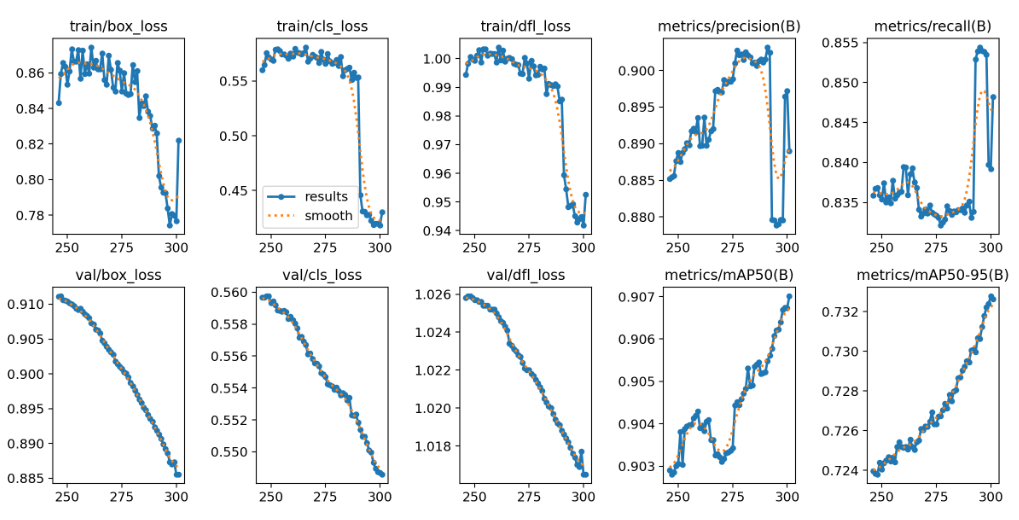
\includegraphics[width=1\textwidth, height=0.3\textheight]{visualize.png}
  \caption{Visualize model.}
  \label{fig:method}
\end{figure}

In the following set of graphs, the val/box loss graph indicates that the bounding box loss in the validation set decreased from 0.910 to approximately 0.885. This indicates that the model not only performed better than the training set, but also generalized better on the validation data. The following graph, "val/cls loss", indicates that the classification loss in the validation set decreased from 0.558 to approximately 0.550. Even though it is not a major drop, it is still showing a positive trend. From the val/dfl loss plot, it is evident that the distribution function loss decreased from 1.026 to around 1.018, making the model more stable in prediction. The last two plots show important key data:
metrics/mAP50(B) shows that average precision at IoU 0.5 improved from 0.907 to approximately 0.910, which is good performance for medium-accuracy object detection. "metrics/mAP50-95(B)" shows that mAP improves from 0.732 to approximately 0.740 between IoU thresholds of 0.5 and 0.95.Object detection performance tends to be better with more restrictive criteria. These plots generally indicate the machine learning model exhibits a trend of improving performance with epochs. The values of loss are decreasing on both the training and validation sets, and the rate of decrease slows down between 250 and 300 epochs. In the meantime, other metrics such as precision, hit rate, and mAP are also rising, albeit not significantly. This slowing down may be a sign that the model is approaching a convergence point, where performance is at an optimal level and does not improve significantly further. This means that further training will not be so effective.

Therefore, the users must try the model at this stage or adjust hyperparameters in a proper manner to achieve further improvements.
The images were preprocessed to 640 x 640. Mirror, 90 degree rotation, grayscale, brightness, exposure, blur, and noise augmentation have been applied. Bounding boxes marking the face boundaries have been marked in all the images and tagged with corresponding class labels of emotion for proper classification and identification. Table 3.1 illustrates the dataset distribution by emotion.

\begin{table}[H]
    \centering
    \caption{Example table with four columns}
    \label{tab:example_table}
    \begin{tabular}{cccc}
        \toprule
        \textbf{Category} & \textbf{Training} & \textbf{Validation} & \textbf{Test} \\
        \midrule
            Anger & 770 & 57 & 99 \\
            Contempt & 855 & 76 & 106 \\
            Disgust & 838 & 80 & 99 \\
            Fear & 652 & 85 & 90 \\
            Happy & 2273 & 214 & 289 \\
            Neutral & 1637 & 186 & 215 \\
            Sad & 925 & 102 & 113 \\
            Surprised & 853 & 117 & 107 \\
        \bottomrule
        \textbf{Total Images} & \textbf{8808} & \textbf{917} & \textbf{1118} \\
    \end{tabular}
\end{table}

\section{Environment Settings}
All experiments were conducted on Google Colab, Kaggle a cloud-based platform with GPU acceleration. The implementation utilized Python 3.12.4 and Torch 2.4.0, leveraging CUDA 12.4 and an NVIDIA Tesla T4 GPU for efficient training and inference. The environment provided 12.7 GB of RAM and 15 GB of GPU memory, sufficient for model training and evaluation. The remaining models besides YOLOv12, we train using kaggle with GPU P100, 16Gb Ram GPU and 15Gb CPU. We still train with the same dataset and settings as training on google colab. Training ran for 120 epochs with a batch size of 32, using 640 × 640 pixel images and defaults set up. This setup ensured computational efficiency and model performance.

\begin{table}[H]
    \centering
    \caption{Example table with four columns}
    \label{tab:example_table}
    \begin{tabular}{cccc}
        \toprule
        \textbf{Category} & \textbf{Training} & \textbf{Validation} & \textbf{Test} \\
        \midrule
            Anger & 770 & 57 & 99 \\
            Contempt & 855 & 76 & 106 \\
            Disgust & 838 & 80 & 99 \\
            Fear & 652 & 85 & 90 \\
            Happy & 2273 & 214 & 289 \\
            Neutral & 1637 & 186 & 215 \\
            Sad & 925 & 102 & 113 \\
            Surprised & 853 & 117 & 107 \\
        \bottomrule
        \textbf{Total Images} & \textbf{8808} & \textbf{917} & \textbf{1118} \\
    \end{tabular}
\end{table}

This is an example of the dataset used to train, test, and validate the emotion recognition model from facial images. The table is divided into four columns: emotion category, number of images used for training, validation, and testing. Eight main emotion categories are classified and labeled: Angry, Contempt, Disgust, Fear, Happy, Neutral, Sad, and Surprised. In the "Training" column, the "Happy" emotion has the highest number of samples with 2,273 images, the "Fear" emotion has the lowest number of samples with 652 images; this contrast can easily affect the accuracy of the model. Similarly, in the Validation and Test columns, the number of images is also evenly distributed among the emotion groups but still maintains a certain difference. A total of 8,808 samples were used for training, 917 samples for validation, and 1,118 samples for testing. Table 1 shows the distribution of input data, ensuring balance and diversity in the data will help the model recognize emotions more accurately and comprehensively in real-world situations.


\begin{figure}[H]
    \centering
    % Hàng trên: 5 ảnh
    \begin{minipage}{0.19\textwidth}
        \centering
        \includegraphics[width=\textwidth,height=0.15\textheight,keepaspectratio]{anger.png} \\ % Ảnh Anger
        \vspace{3pt}
        \small Anger
    \end{minipage}
    \hfill
    \begin{minipage}{0.19\textwidth}
        \centering
        \includegraphics[width=\textwidth,height=0.15\textheight,keepaspectratio]{contempt.png} \\ % Ảnh Contempt
        \vspace{3pt}
        \small Contempt
    \end{minipage}
    \hfill
    \begin{minipage}{0.19\textwidth}
        \centering
        \includegraphics[width=\textwidth,height=0.13\textheight,keepaspectratio]{disgust.png} \\ % Ảnh Disgust
        \vspace{3pt}
        \small Disgust
    \end{minipage}
    \hfill
    \begin{minipage}{0.19\textwidth}
        \centering
        \includegraphics[width=\textwidth,height=0.13\textheight,keepaspectratio]{fear.png} \\ % Ảnh Fear
        \vspace{3pt}
        \small Fear
    \end{minipage}
    \hfill
    \begin{minipage}{0.19\textwidth}
        \centering
        \includegraphics[width=\textwidth,height=0.13\textheight,keepaspectratio]{happy.png} \\ % Ảnh Happy
        \vspace{3pt}
        \small Happy
    \end{minipage}

    \vspace{10pt} % Khoảng cách giữa hai hàng

    % Hàng dưới: 4 ảnh, sát vào nhau, ảnh cuối to hơn
    \begin{minipage}{0.19\textwidth}
        \centering
        \includegraphics[width=\textwidth,height=0.15\textheight,keepaspectratio]{neutral.png} \\ % Ảnh Neutral
        \vspace{3pt}
        \small Neutral
    \end{minipage}
    \hspace{5pt} % Khoảng cách nhỏ giữa các ảnh
    \begin{minipage}{0.19\textwidth}
        \centering
        \includegraphics[width=\textwidth,height=0.15\textheight,keepaspectratio]{sad.png} \\ % Ảnh Sad
        \vspace{3pt}
        \small Sad
    \end{minipage}
    \hspace{5pt}
    \begin{minipage}{0.19\textwidth}
        \centering
        \includegraphics[width=\textwidth,height=0.15\textheight,keepaspectratio]{surprised.png} \\ % Ảnh Surprised
        \vspace{3pt}
        \small Surprised
    \end{minipage}
    \hspace{5pt}
    \begin{minipage}{0.24\textwidth} % Tăng chiều rộng để ảnh to hơn
        \centering
        \includegraphics[width=\textwidth,height=0.15\textheight,keepaspectratio]{many faces.png} \\ % Ảnh Many Faces
        \vspace{3pt}
        \small Many Faces
    \end{minipage}

    \vspace{10pt} % Khoảng cách trước chú thích tổng thể
    \caption{Emotion List} % Chú thích tổng thể với "Figure"
    \label{fig:emotion_list}
\end{figure}


% \begin{table}[h]
%   \centering
%   \caption{Data Sources}
%   \label{tab:data}
%   \begin{tabular}{lcc}
%     \toprule
%     Source & Type & Year \\
%     \midrule
%     [Source 1] & Primary & 2024 \\
%     [Source 2] & Secondary & 2023 \\
%     \bottomrule
%   \end{tabular}
% \end{table}

\section{Evaluation Metrics}
To assess the product detection performance of YOLO models in the checkout system, we employed Precision, Recall, and Mean Average Precision (mAP) as main evaluation metrics. Precision evaluates the proportion of correct detections to all detections, basically eliminating false positives. Recall assesses the proportion of correctly detected products to all existing products, reducing missed detections. mAP, as the average of Average Precision (AP) over all product categories, provides a broad sense of model accuracy. Specifically, mAP@0.5 uses an IoU of 0.5 to quantify straightforward detection accuracy, and mAP@0.5:0.95 averages AP over IoU thresholds ranging from 0.5 to 0.95 in increments of 0.05 for a stricter testing of detection and localization accuracy. Taken together, these metrics offer a robust evaluation of the performance and reliability of the YOLO models in real-time detection of products.

%\begin{itemize}
 % \item Preprocessing with [tool].
  %\item Analysis using [method].
  %\item Evaluation via [metrics].
%\end{itemize}


% Chapter: Results & Discussions
\clearpage
\chapter{RESULTS \& DISCUSSIONS}
\section{Results}
Table 4.1 is the result we trained with 5 different YOLO versions to compare the results between versions with the latest version we used, YOLOv12.

\begin{table}[H]
    \centering
    \caption{Evaluation results of YOLO models}
    \label{tab:yolo_evaluation}
    \begin{tabular}{lccccc}
        \toprule
        \textbf{Model} & \textbf{Params (M)} & \textbf{P} & \textbf{R} & \textbf{mAP@0.5} & \textbf{mAP@0.5:0.95} \\
        \midrule
        YOLOv12s & 9.26 & 0.937 & 0.898 & 0.941 & 0.851 \\
        YOLOv11s & 9.46 & 0.942 & 0.898 & 0.935 & 0.833 \\
        YOLOv10s & 8.04 & 0.923 & 0.874 & 0.935 & 0.813 \\
        YOLOv9s  & 7.29 & 0.938 & 0.867 & 0.936 & 0.807 \\
        YOLOv8s  & 11.14 & 0.897 & 0.835 & 0.909 & 0.741 \\
        \bottomrule
    \end{tabular}
\end{table}

YOLOv12s achieves the highest mAP@0.5 (0.941) with strong Precision (0.937) and Recall (0.908), indicating robust detection of facial emotions at a more lenient IoU threshold. However, its mAP@0.5:0.95 (0.851) suggests weaker localization at stricter thresholds. YOLOv10s, with fewer parameters (8.04M), outperforms others in mAP@0.5:0.95 (0.813) while maintaining competitive Precision (0.923) and Recall (0.874), highlighting superior robustness in precise emotion localization. YOLOv9s, the lightest model at 7.29M parameters, shows a balanced performance with mAP@0.5: 0.936 and mAP@0.5:0.95: 0.807, offering efficiency without sacrificing accuracy. YOLOv11s (P: 0.942, R: 0.898, mAP@0.5: 0.935, mAP@0.5:0.95: 0.833) provides a stable trade-off, though its lower Recall may miss some emotions. YOLOv8s, despite having the most parameters (11.14M), underperforms with the lowest mAP@0.5: 0.909 and mAP@0.5:0.95: 0.741, suggesting limited gains in facial emotion recognition, particularly in precise localization.

\section{Measuring performance}
Evaluating the performance of the YOLO model in the task of facial emotion detection, we used the metrics Precision, Recall, mAP@0.5, and mAP@0.5:0.95 on the test set consisting of 917 images with 2820 samples. Table 3 below shows the results for each class.

\begin{table}[H]
    \centering
    \caption{YOLOv12 evaluation metrics per class}
    \label{tab:yolov12_metrics}
    \begin{tabular}{lcccccc}
        \toprule
        \textbf{Class} & \textbf{Images} & \textbf{Instances} & \textbf{Box(P)} & \textbf{R} & \textbf{mAP50} & \textbf{mAP50-95} \\
        \midrule
        All       & 917  & 2820 & 0.937 & 0.898 & 0.941 & 0.851 \\
        Anger     & 96   & 151  & 0.953 & 0.887 & 0.933 & 0.838 \\
        Contempt  & 112  & 133  & 0.955 & 0.947 & 0.964 & 0.932 \\
        Disgust   & 89   & 138  & 0.981 & 0.928 & 0.952 & 0.908 \\
        Fear      & 88   & 139  & 0.938 & 0.882 & 0.902 & 0.813 \\
        Happy     & 209  & 197  & 0.934 & 0.888 & 0.944 & 0.751 \\
        Neutral   & 216  & 681  & 0.917 & 0.827 & 0.908 & 0.763 \\
        Sad       & 105  & 199  & 0.955 & 0.905 & 0.981 & 0.906 \\
        Surprised & 117  & 182  & 0.863 & 0.934 & 0.94  & 0.888 \\
        \bottomrule
    \end{tabular}
\end{table}

The overall results demonstrate that our model reached a Precision of 0.937, which means that 93.7\% of the predictions And they reclassify non-symptomatic cases, ensuring that only truly symptomatic cases are counted, to reduce the chance of false detections. Recall was 0.898, meaning that the model detected 89.8\% of every faces gushing real emotions with hardly none left out. The mAP@0.5 (0.941) was reached for the last index, implying high mAP at IoU 0.5, and the mAP@0.5:0.95 converged to 0.851, showing good detection and localization at different IoU thresholds from 0.5 to 0.95. The model demonstrates many noteworthy strengths. First of all, the overall performance is very impressive with Precision reaching (0.937), Recall (0.898), mAP@0.5 (0.941), and mAP@0.5:0.95 (0.851), demonstrating the ability to detect and locate accurately on the test set of 2820 samples. Especially, classes such as Contempt mAP@0.5 (0.964), mAP@0.5:0.95 (0.932) and Sad mAP@0.5 (0.981), mAP@0.5:0.95 (0.906) achieved outstanding results, demonstrating that the model performs effectively with classes that have clear expressive features. This may be due to the application of data augmentation techniques such as flipping, rotating, and adjusting brightness, which help the model learn diverse features.

However, the model also reveals some weaknesses. The Happy class has the lowest mAP@0.5:0.95 (0.751), despite having the largest number of samples (1197), indicating difficulties in precise localization due to the diversity and complexity of joyful expressions, especially in group photos. Similarly, the Neutral class (mAP@0.5:0.95 0.763, Recall 0.827) and the Fear class (mAP@0.5:0.95 0.813) have lower performance, possibly due to the similarity in features between these classes and others, leading to confusion. Additionally, the Surprised class has the lowest Precision (0.863), indicating a high false detection rate, due to the training data not being sufficiently representative of this class.

The model is capable of accurately detecting basic emotions and thanks to the use of advanced deep learning algorithms, the system has achieved high accuracy on the test data set, reflecting the outstanding recognition efficiency compared to previous models. In addition, the real-time recognition feature has been integrated and operated stably on the web platform, using the WebSocket protocol to ensure fast, slow transmission speed and smooth user experience. Users can adjust the reliability level of the information recognition results via the slider on the interface, allowing for personalization and system adjustment.

On the mobile platform, the model is optimized, the Android version is developed using the TensorFlow Lite library, which helps to process directly on the device, ensuring stable and high performance, enhancing security and privacy for users. Regarding the application features, there are currently several functions such as selecting available images, taking photos directly via the camera and analyzing videos.

\section{Intergrated into a cross – platform application }
\subsection{Overview of functions}
Multi-platform emotion recognition aims to be simple and friendly, giving users an easy way to analyze emotions from images, videos, or their webcam. The screen has a confidence score slider—move it up or down to make the emotion results more accurate. Plus, the real-time emotion feature with your webcam will soon be connected to an AI chatbot. This chatbot will automatically chat with you in a style tailored to how you’re feeling at the moment. You can message and talk with the AI bot directly too, with responses happening on the fly. The interface keeps things straightforward: four main functions and clearly labeled navigation buttons make it easy to use and find what you need.\\

\begin{figure}[H]
  \centering
  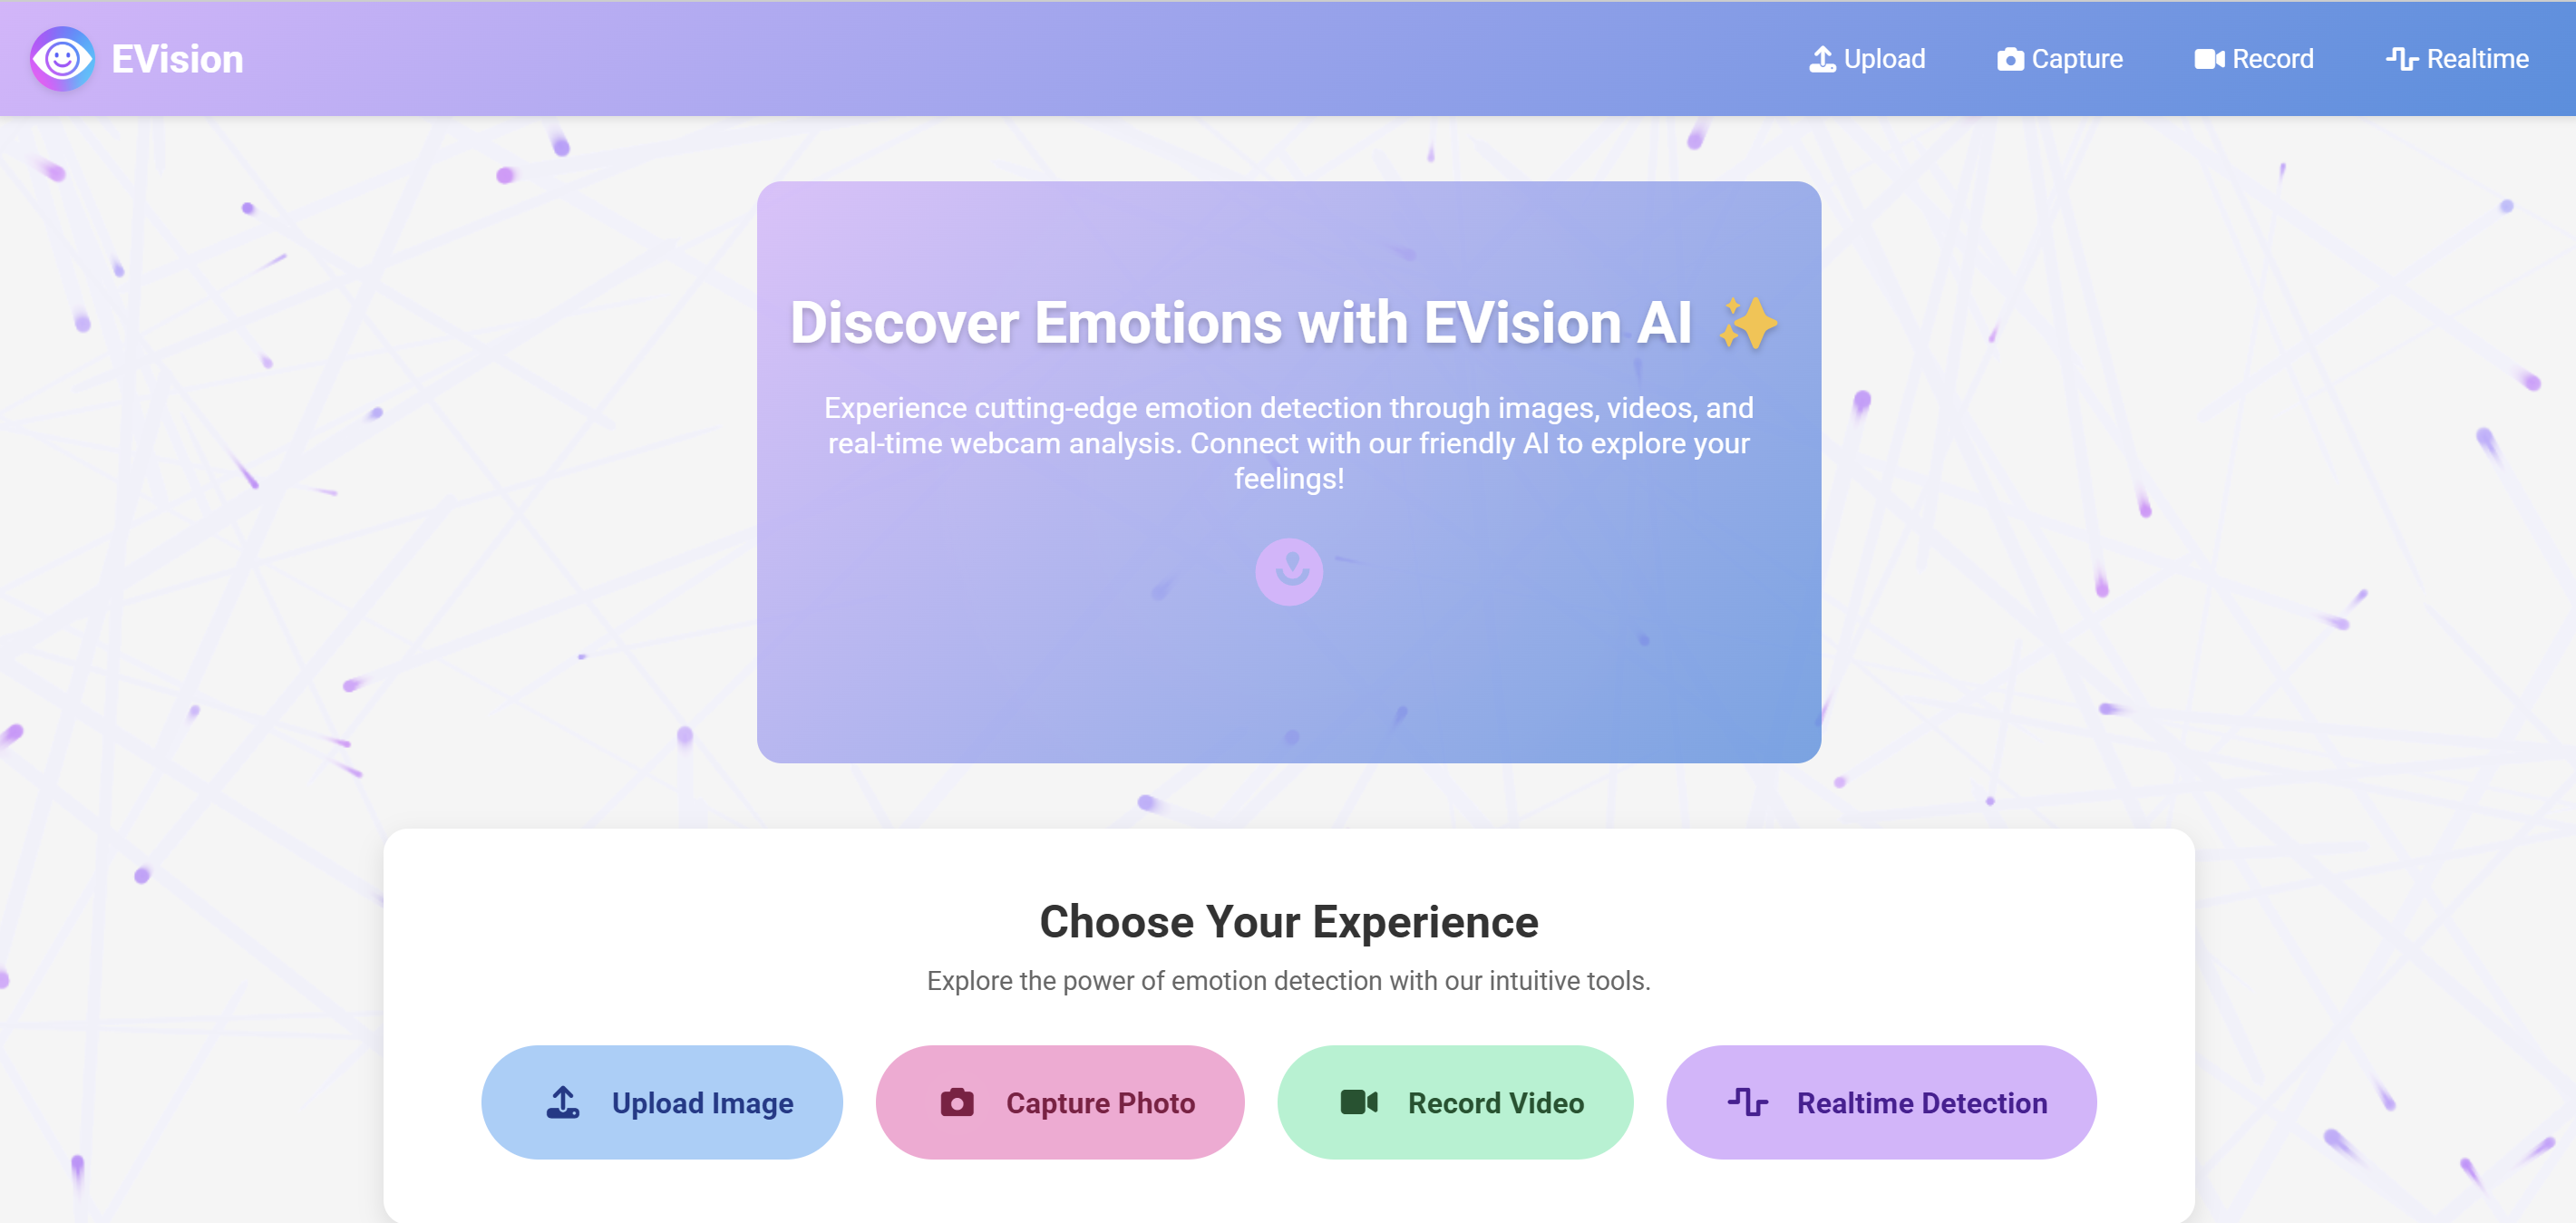
\includegraphics[width=0.8\textwidth]{web home page.png}
  \caption{Web home page}
  \label{fig:method}
\end{figure}


This first function will help the users in uploading the photos from the library for emotion recognition as they can upload the images from their personal devices. By clicking the upload button, then the user will select an image file selected in input file field and sent a request to server. The image is processed, a call is made to the emotion recognition model and the result is returned as text along with emotion name, confidence score and data about the processed image with the emotion label. Users can slide a slider bar to adjust the confidence threshold; thus, the recognition results can be adjusted or tuned to an acceptable range of accuracy.

\begin{figure}[H]
  \centering
  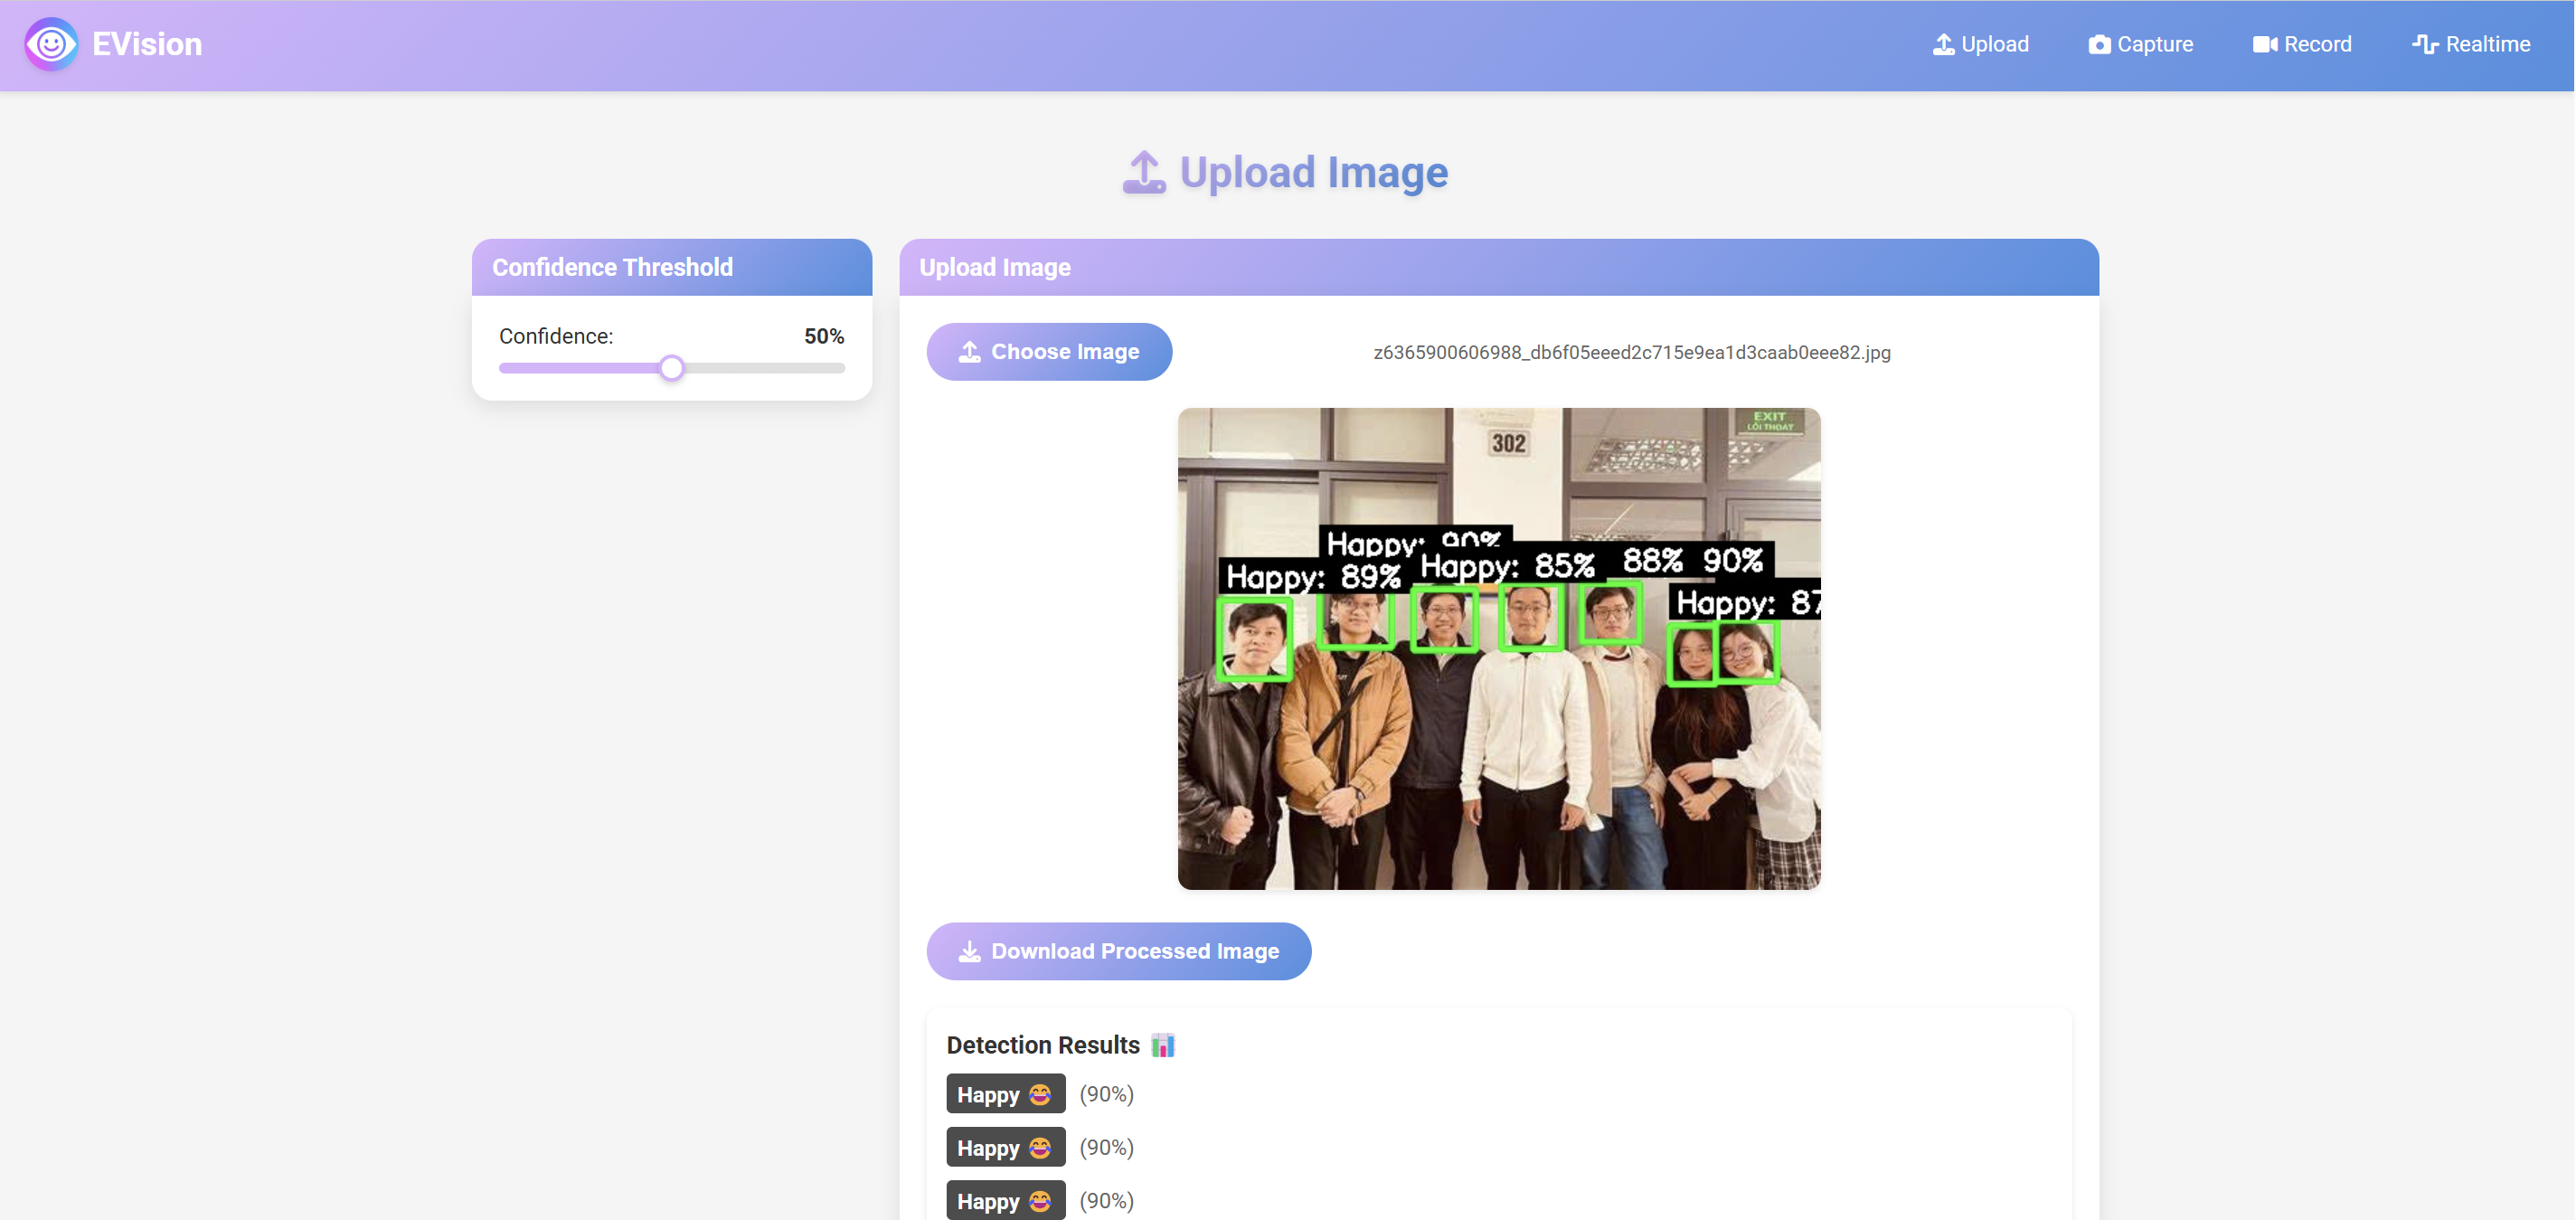
\includegraphics[width=0.8\textwidth]{web image upload function.png}
  \caption{Web image upload function}
  \label{fig:result}
\end{figure}

\begin{figure}[H]
  \centering
  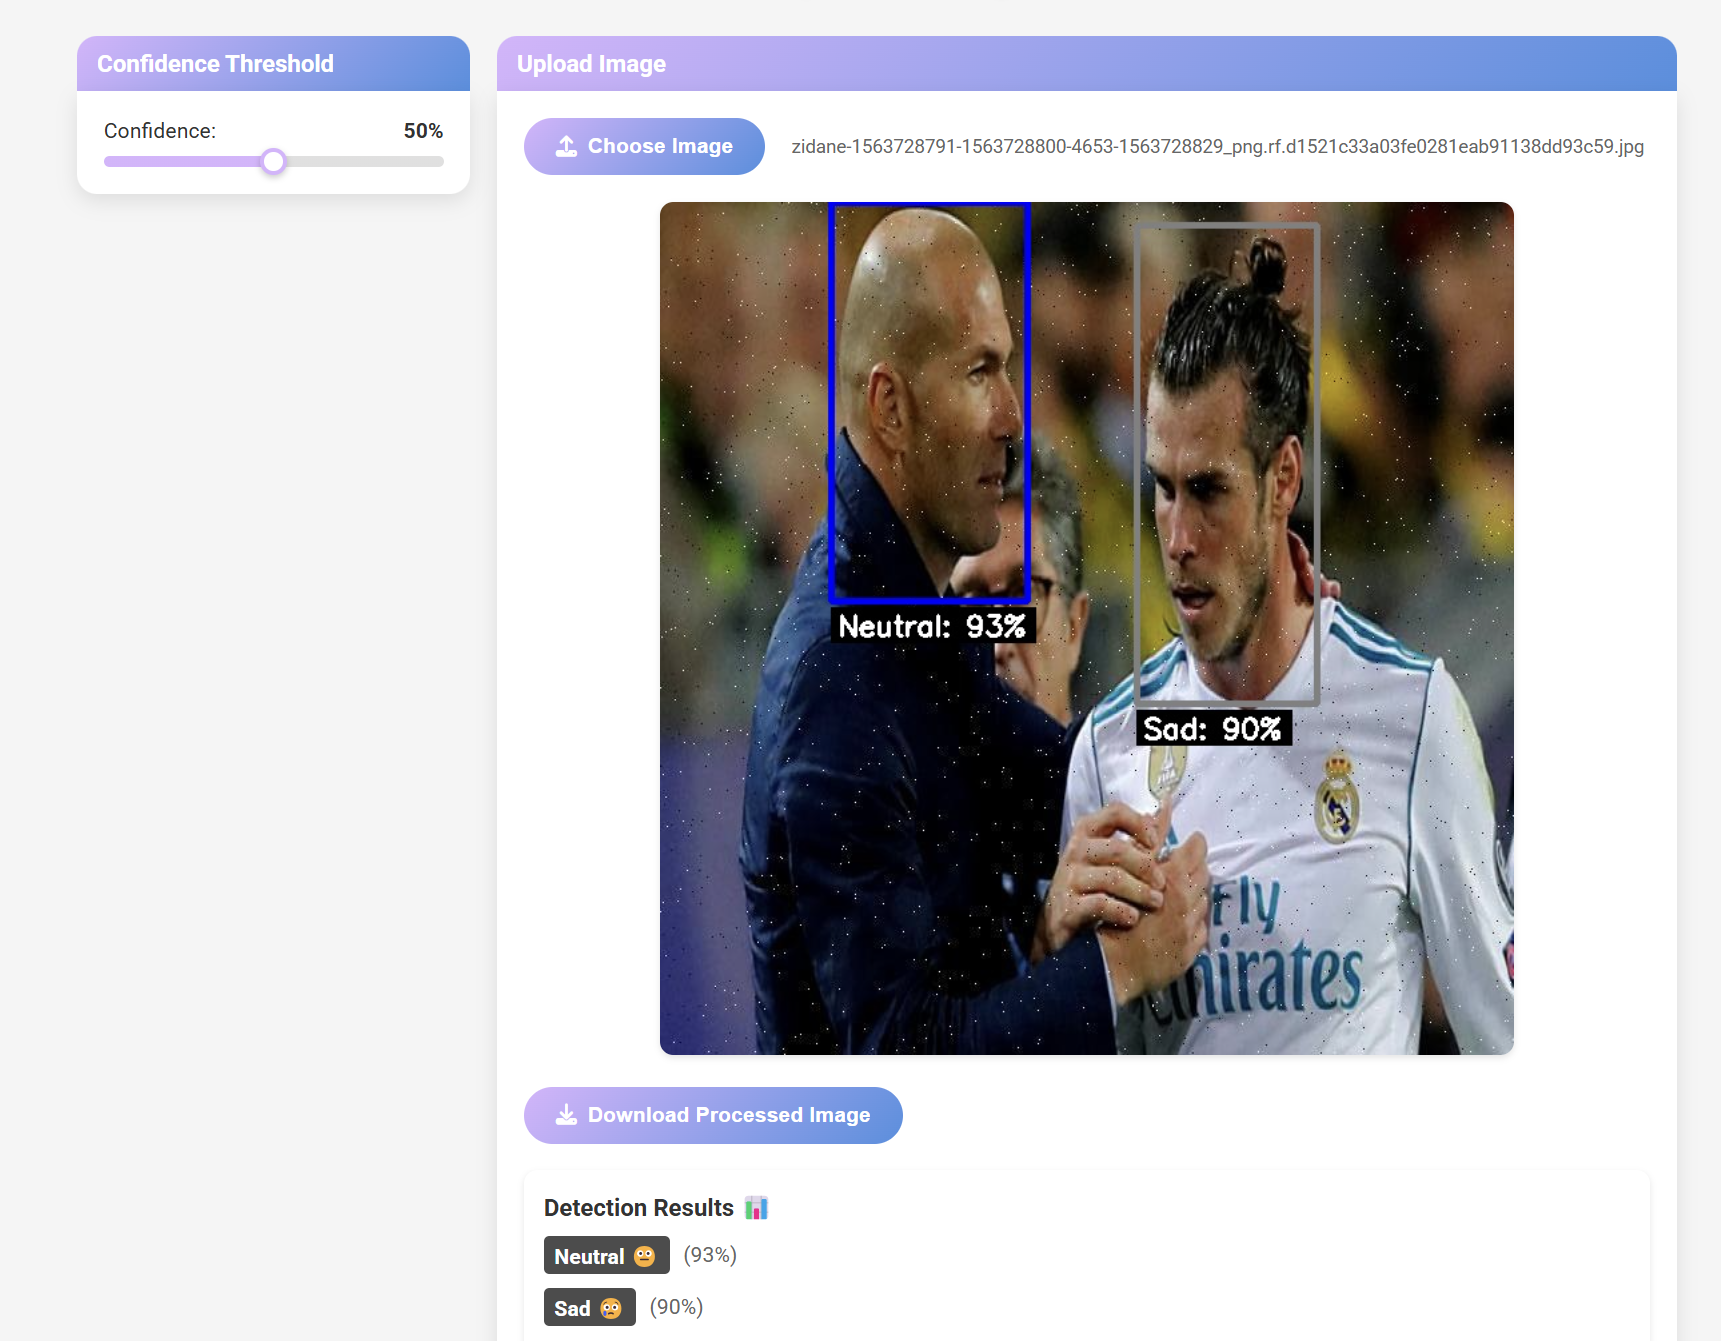
\includegraphics[width=0.8\textwidth]{web image upload function 1.png}
  \caption{Web image upload function}
  \label{fig:result}
\end{figure}

The second function is to get photos from the webcam which is supposed to grab pictures directly from the user’s webcam. A reliability adjusted button to take photos is offered with a computer webcam display area. This will be a function to send the snapshots in server and recognise emotions as snap like file uploads being used for the cases where quick analysis is needed without file uploading.

\begin{figure}[H]
  \centering
  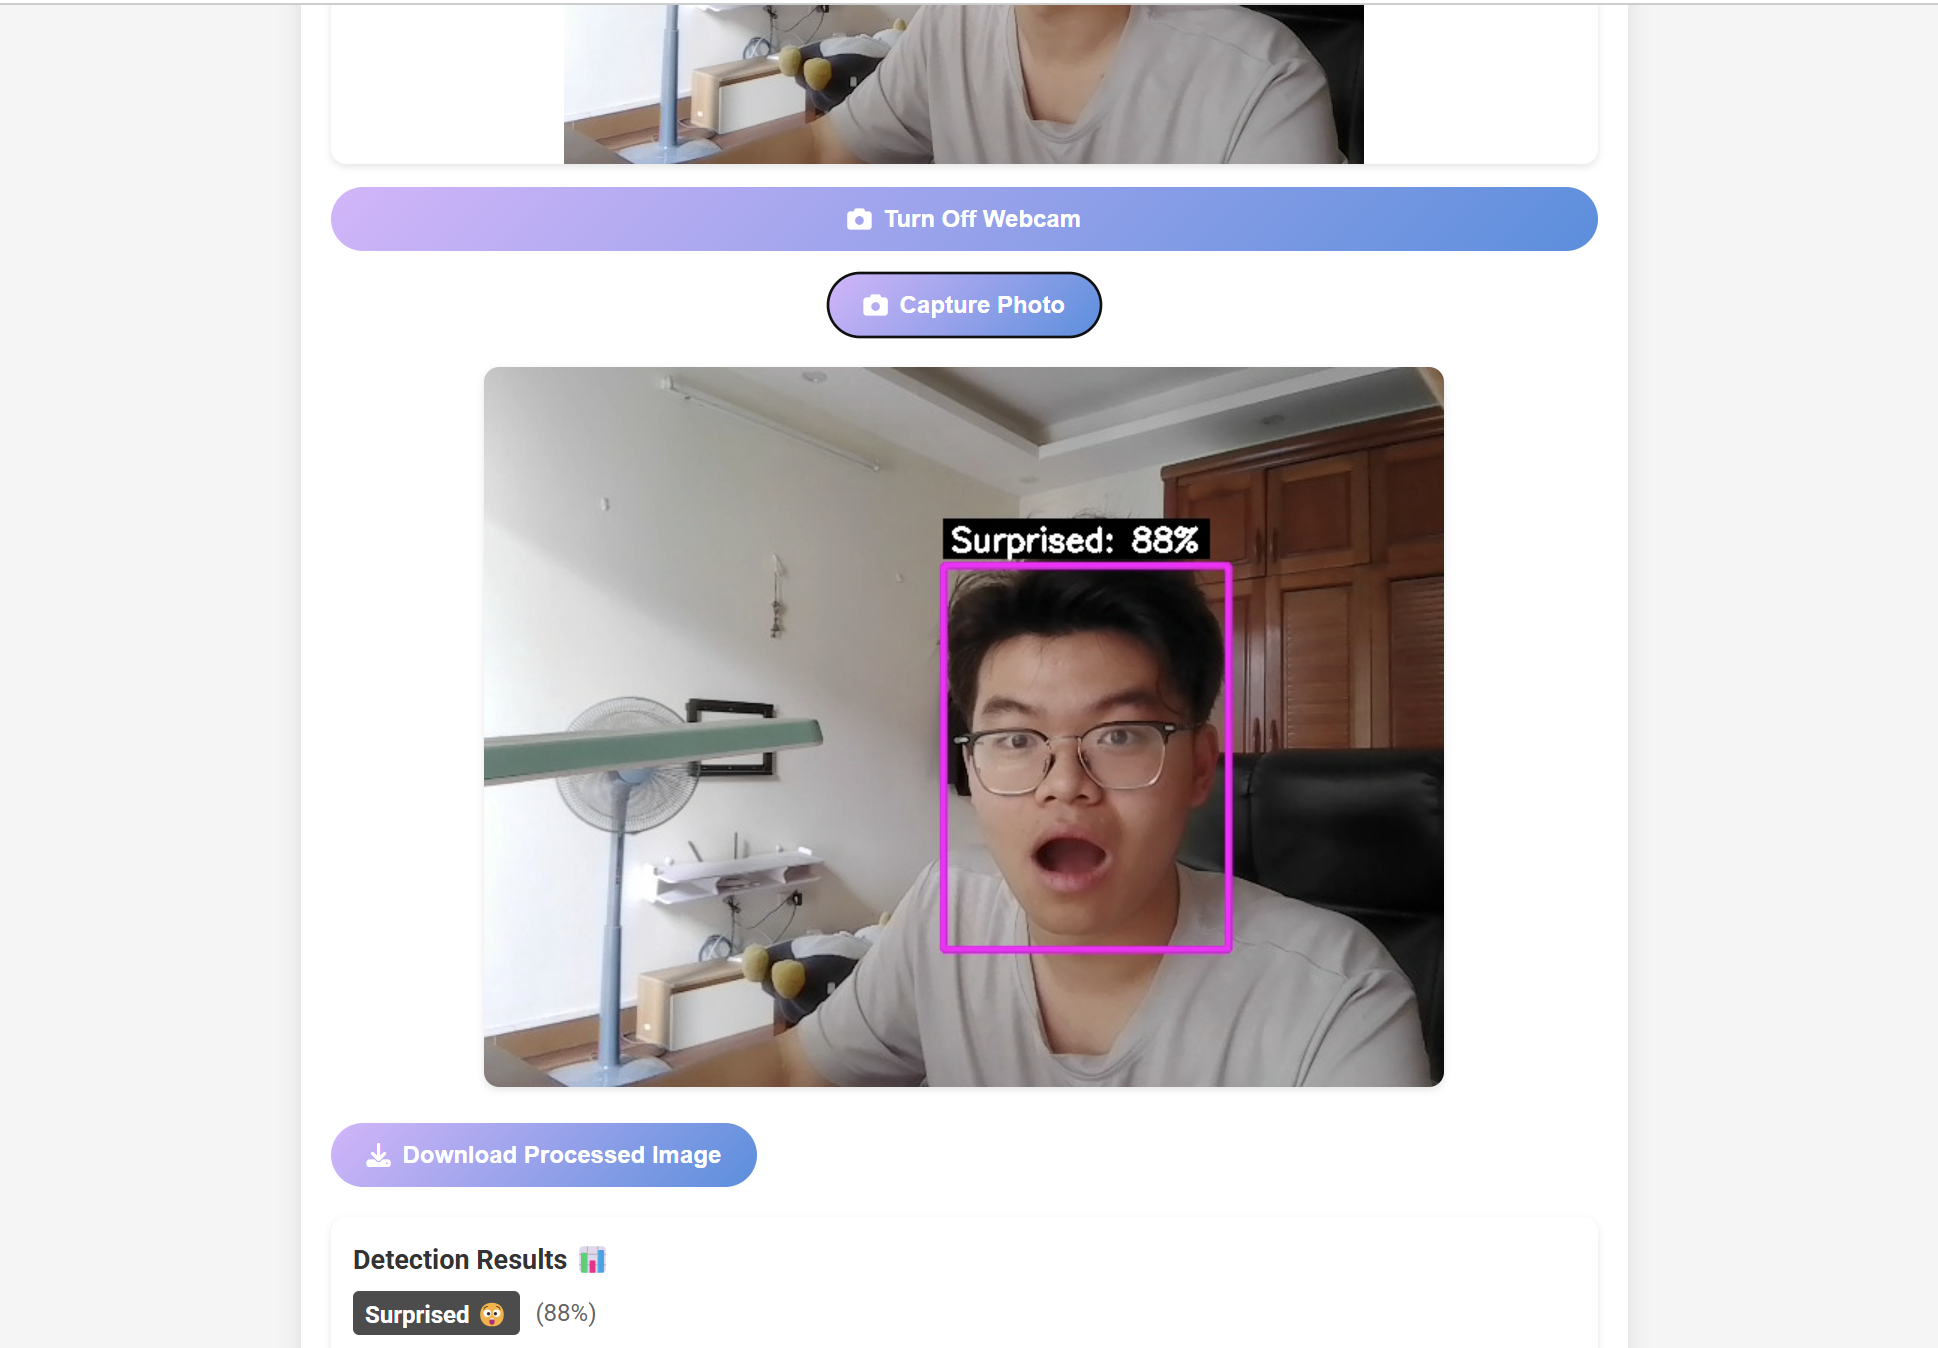
\includegraphics[width=0.8\textwidth]{Webcam capture function.png}
  \caption{Webcam capture function}
  \label{fig:method}
\end{figure}

\newpage Video recording is done for emotion extraction from webcam captured videos, which is the third function provided by the software. In the same way as taking photos, the interface has a webcam entry and an ability to fix dependability. This function can be utilized to record a short video and send it to the server for real time or aggregated emotion analysis, as well as expanded for the use in scenarios as interviews or emotional monitoring.

\begin{figure}[H]
  \centering
  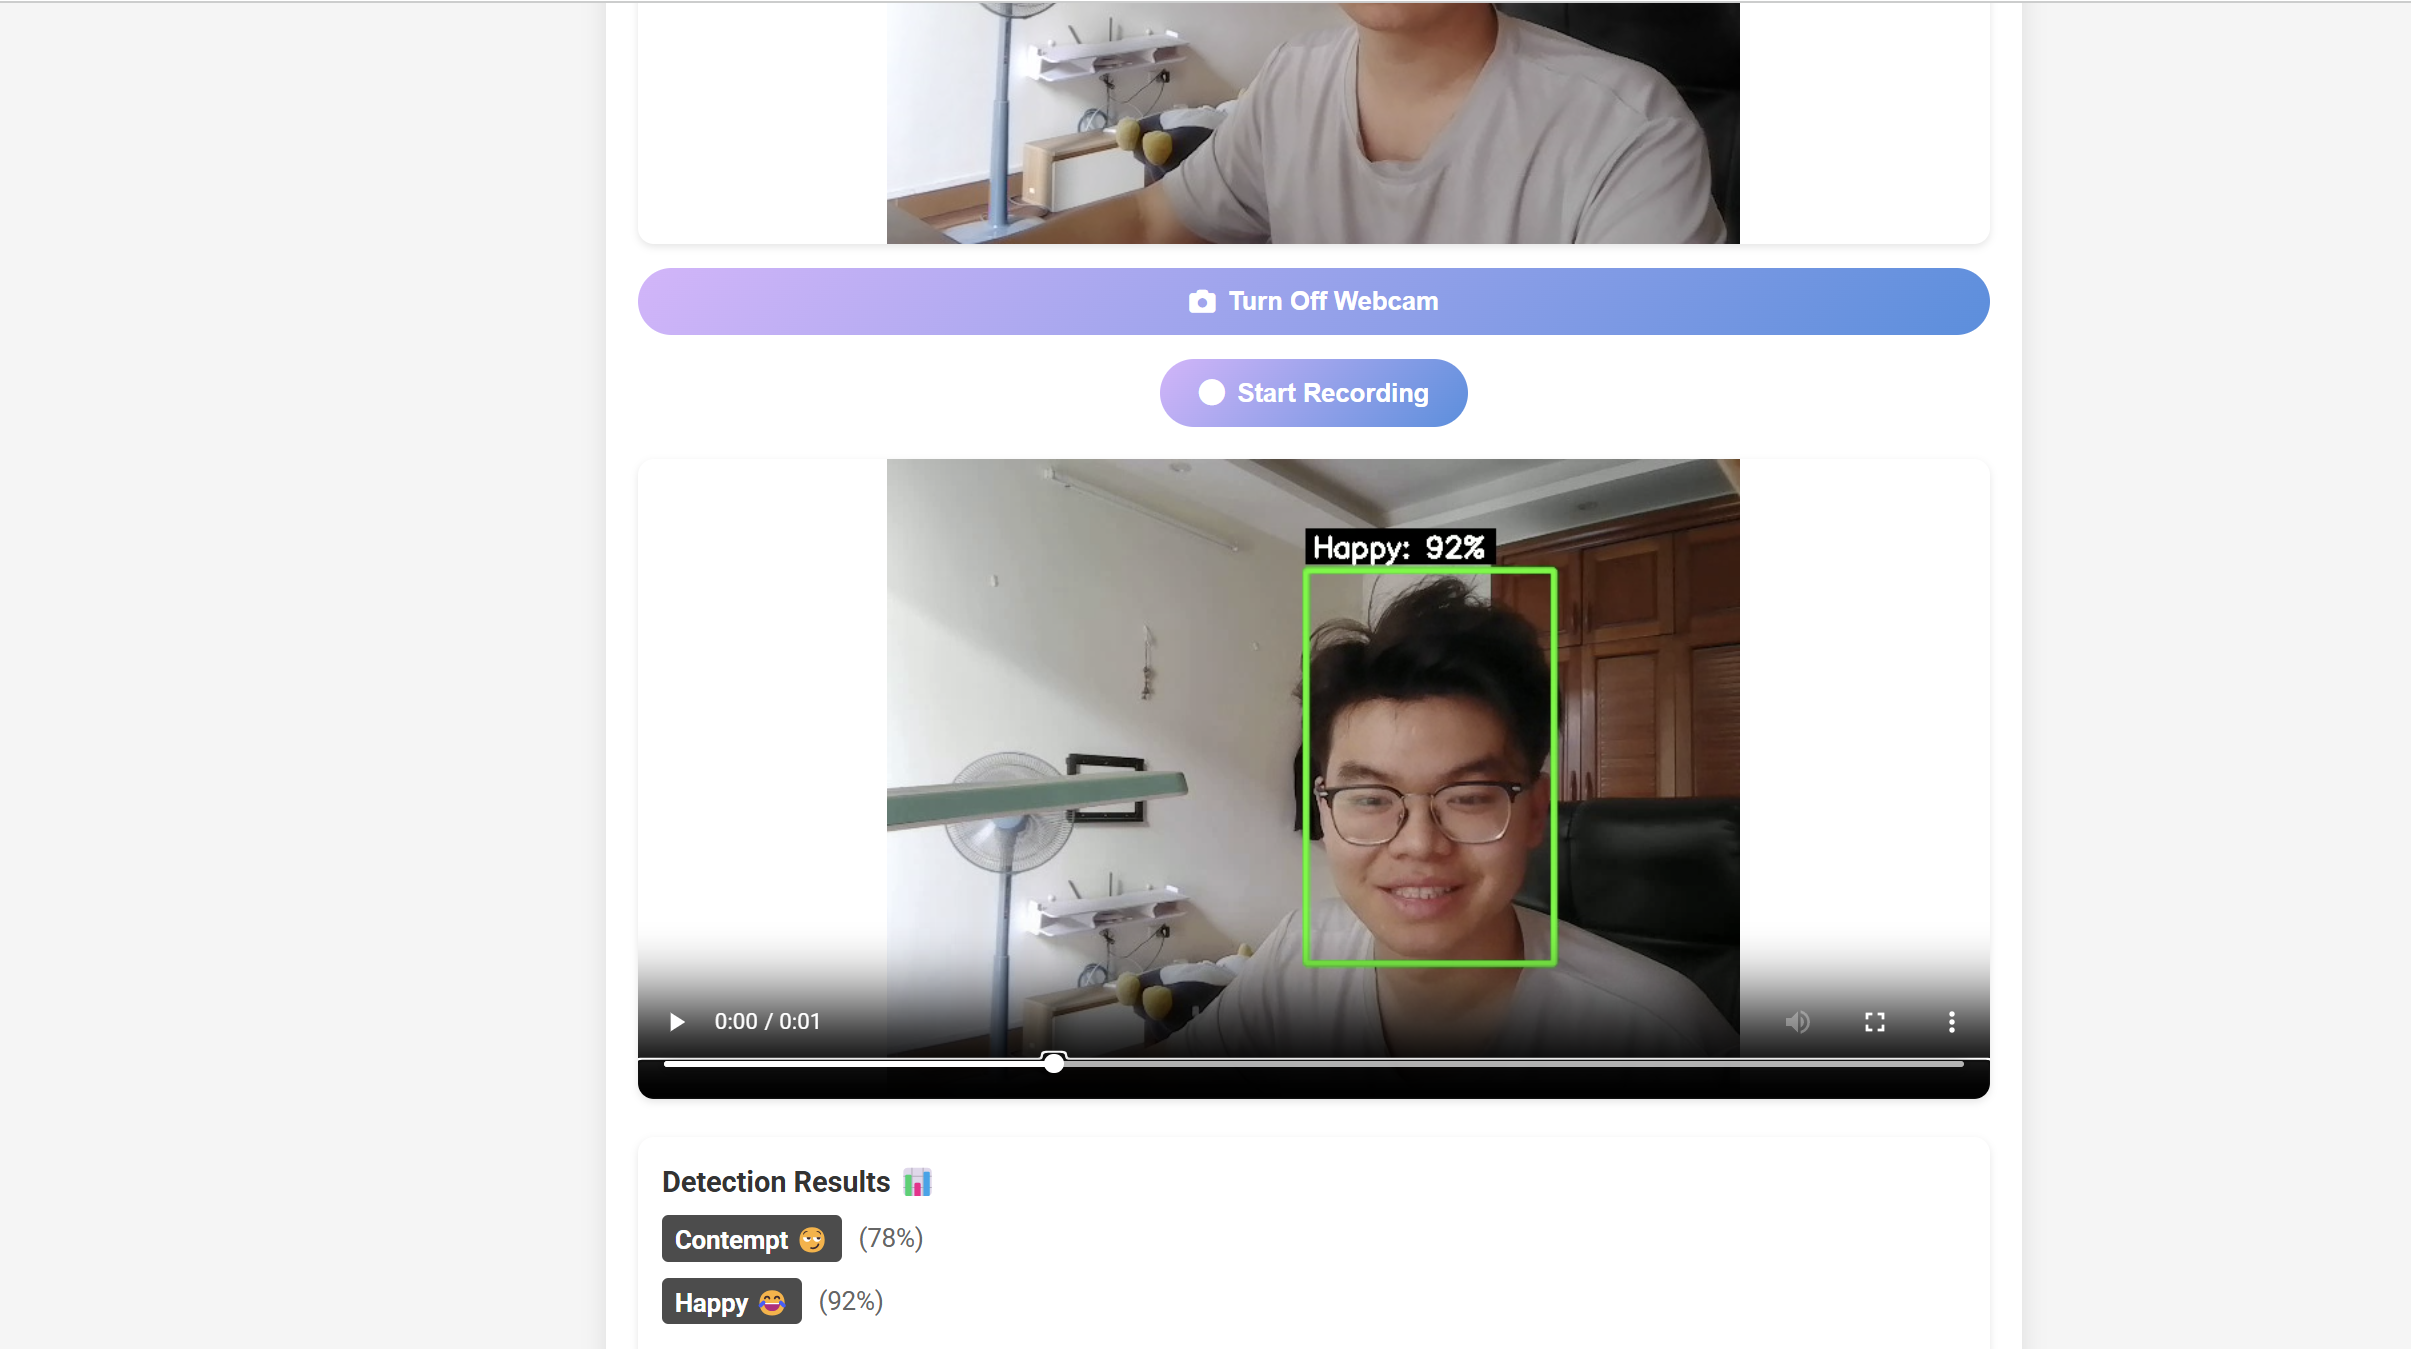
\includegraphics[width=0.8\textwidth]{webcam video capture.png}
  \caption{webcam video record}
  \label{fig:method}
\end{figure}

This is the fourth and most advanced real time function which allows for continuous emotion analysis of the webcam video stream. On the other hand, it draws live video from the webcam on a canvas and overlays real time emotion labels in a canvas. There is a dedicated button for the turning on/off the webcam, and the reliability is changed through a slider. However, when the reliability is even minutely fine tuned, the results and bounding boxes will adjust their accuracy only after some delay. WebSocket is used to send frames to the server periodically, receive results and immediately update interface. This feature also allows the addition of and AI chatbot for users to chat and be fed back based on detected emotions, forming a unique interactive experience.

\begin{figure}[H]
  \centering
  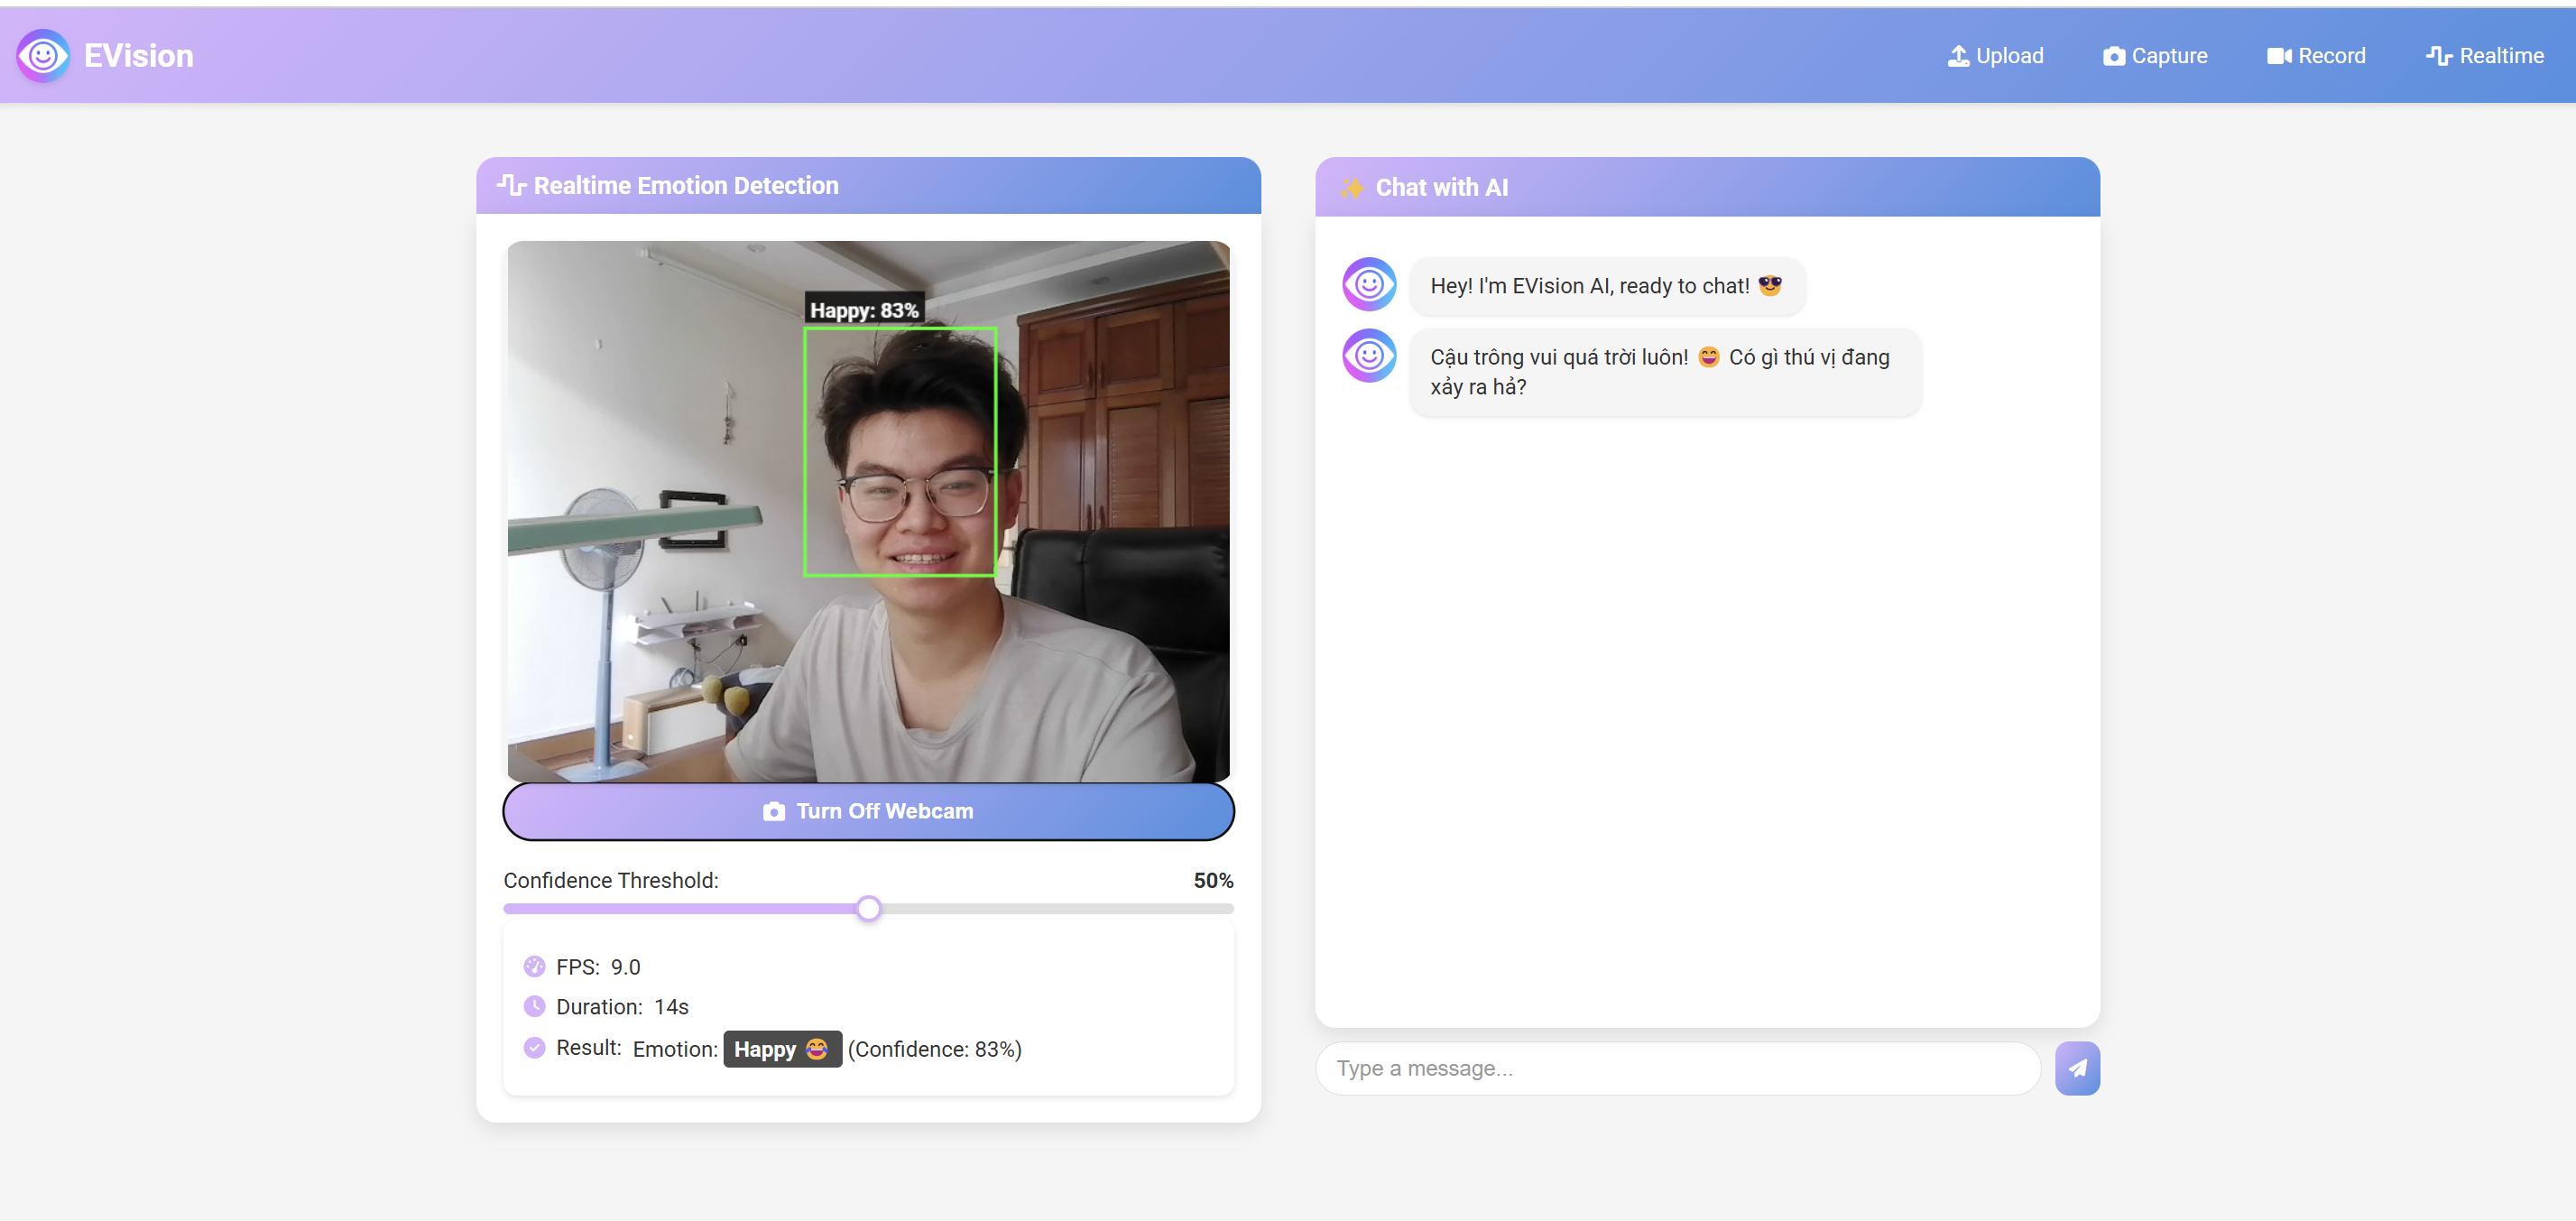
\includegraphics[width=0.8\textwidth]{Realtime webcam chatbot.png}
  \caption{Realtime webcam chatbot}
  \label{fig:method}
\end{figure}

EVision's webcam scans and analyzes the user's image, printing out the "Happy" emotion result - 50\% accurate.

\begin{figure}[H]
  \centering
  \includegraphics[width=0.8\textwidth]{Realtime webcam chatbot 1.png}
  \caption{Realtime webcam chatbot}
  \label{fig:method}
\end{figure}

EVision's webcam scans and analyzes the user's image, printing out the "contempt" emotion result - 87\% accurate.


\subsection{Web}
The web application is built using Flask, a lightweight Python framework that supports backend processing such as routing and handling HTTP requests. The frontend uses JavaScript along with HTML and CSS to design the user interface.

\subsubsection{3.2.1 Set up the enviroment}
The system uses Python 3.11 with a virtual environment activated for managing libraries in isolation in order to avoid conflicts for the purposes of deploying the emotion recognition web application. The main framework used for backend is the Flask--2.3.2 in order to handle routes and render templates. Firstly, to support image processing before the input, the Opencv-python--4.8.0.76 library is added, followed by Torch--2.6.0, Torchvision--0.26.0, Ultralytics--8.3.107 to help load the model and identify the emotions. In order to perform array operations in the data processing, they use NumPy–1.26.0. Flask-SocketIO–5.3.4 is used to provide WebSockets support for real-time recognition functions and Werkzeug–3.1.3 is used to ensure that user uploaded files are safely handled. Templates/ directory where all HTML files to create the web framework are, static directory where the CSS and JavaScript files to design the user interface and handle user tasks are present in. Python files to load the PyTorch model and drawing the bounding boxes are put in the src/ directory. Next, it will contain app.py file for Flask logic that completes the project and the web in the root directory. This will set up and run the environment to Localhost. 
This process ensures that the environment is fully set up, ready for the development and testing of emotion recognition features.

\subsubsection{3.2.2 Content of deployment }
The /upload route is created during the implementation process to handle POST requests carrying image files from the users using the Werkzeug library to protect the files while processing. First of all, the images are preprocessed using OpenCV, that is, converted to grayscale or resized, before feeding them into the emotion recognition model built using PyTorch. It takes the model, which predicts emotions along with confidence levels and returns the results in JSON format of emotion information, confidence percentages and processed images with bounding boxes drawn on the faces. The result is sent back to the frontend where pure javascript updates the dynamic interface to represent the information visually. Figure 4.8 below illustrates how web can detect an emotion from the input images.

% Đảm bảo các hình trước đó không ảnh hưởng
\FloatBarrier

\begin{figure}[H] % Ép buộc vị trí tại đây
  \centering
  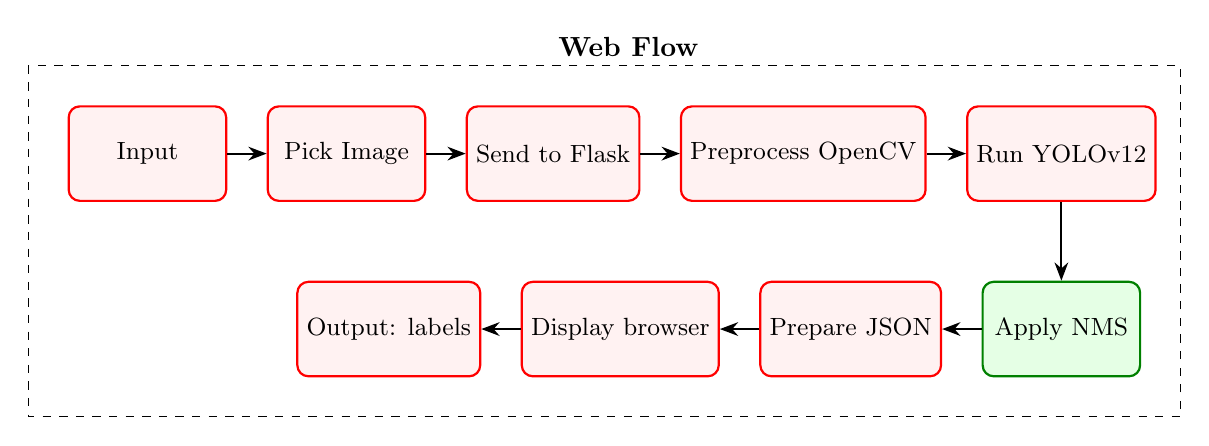
\begin{tikzpicture}[
    node distance=1cm and 0.5cm, % Giảm khoảng cách để vừa trang
    box/.style={
      rectangle,
      rounded corners,
      minimum height=1.2cm,
      minimum width=2cm, % Giảm chiều rộng để vừa trang
      fill=pink!20,
      draw=red,
      thick,
      align=center,
      font=\small
    },
    nms/.style={
      box,
      draw=green!50!black,
      fill=green!10
    },
    arrow/.style={
      -Stealth,
      thick
    }
  ]

  % Các node - Hàng trên
  \node[box] (input) {Input};
  \node[box, right=of input] (pick) {Pick Image};
  \node[box, right=of pick] (flask) {Send to Flask};
  \node[box, right=of flask] (preprocess) {Preprocess OpenCV};
  \node[box, right=of preprocess] (yolo) {Run YOLOv12};

  % Hàng dưới - Căn giữa thủ công
  \node[nms, below=of yolo] (nms) {Apply NMS}; % Dịch sang phải 1cm để căn giữa
  \node[box, left=of nms] (json) {Prepare JSON};
  \node[box, left=of json] (display) {Display browser};
  \node[box, left=of display] (output) {Output: labels};

  % Các mũi tên
  \draw[arrow] (input) -- (pick);
  \draw[arrow] (pick) -- (flask); % Mũi tên giữa Pick Image và Send to Flask thẳng hàng
  \draw[arrow] (flask) -- (preprocess);
  \draw[arrow] (preprocess) -- (yolo);
  \draw[arrow] (yolo) -- (nms); % Mũi tên đi xuống
  \draw[arrow] (nms) -- (json); % Mũi tên ngược lại sang trái
  \draw[arrow] (json) -- (display); % Mũi tên tiếp tục sang trái
  \draw[arrow] (display) -- (output); % Mũi tên tiếp tục sang trái

  % Tiêu đề - Căn giữa thủ công
  \node[above=0.5cm of yolo, xshift=-5.5cm, font=\bfseries] {Web Flow}; % Dịch sang trái 2cm để căn giữa

  % Viền ngoài
  \draw[dashed] ([xshift=-0.5cm, yshift=0.5cm]input.north west) rectangle ([xshift=0.5cm, yshift=-0.5cm]nms.south east);

  \end{tikzpicture}
  \caption{Web Flowchart}
  \label{fig:web_flow}
\end{figure}

% Ngăn các hình sau quay ngược lên trên
\FloatBarrier

Thus, the webcam photo capture function is linked to the /capture route and renders an HTML interface where users can turn on the webcam, take a photo and send the captured images to the server with a POST request like /upload. To analyze emotions, the processing logic will use the PyTorch model, draw bounding boxes on images with OpenCV and return those to the user. Short video clips will be handled by this route that will analyze emotions frame by frame or in aggregate using techniques like batch processing to improve performance.

The web application’s highlight is the real time recognition feature, bound to the /realtime route. This route sets up a Flask-SocketIO WebSocket connection and frames from webcam are sent to the server in real time. navigator.mediaDevices.getUserMedia is used by the frontend to gain access to the webcam and display the live video on a tag and to draw bounding boxes on a face on the tag. Also each class is assigned a unique color for the bounding boxes. The server receives each frame through WebSocket, and OpenCV and the PyTorch model process it to predict the emotions. This results in immediate return of the results, with no delay when the user changes the confidence slider. It is a slider on the frontend that is processed with JavaScript to pass the new confidence value to the server, so that the model can re-fit the bounding box and emotion labels without pausing the video stream.


One of the standout features is in integrating the AI chatbot into real-time functionality. The chatbot uses the gemini-1.5-pro-latest API. In realtime.html, the chatbot is deployed through a chat interface and messages are sent and received using WebSocket. It takes this information from the video stream and makes use of it in order to adjust its chatbot tone – encouraging words for sadness, cheerful questions for happiness. It is easy to build the logic of the chatbot using simple rules:
 'Happy': {
       	 'initial': "You look so happy, is there something interesting going on?",
  	 'tone': "cheerful, humorous, often joking, frequently using the word 'haha' and happy emojis"}. Some responses from chatbot:

\begin{figure}[H]
  \centering
  \includegraphics[width=0.8\textwidth]{Prompt.png}
    \includegraphics[width=0.8\textwidth]{Prompt1.png}
  \caption{Chatbot Responses}
  \label{fig:method}
\end{figure}

The explanation: after we enable the webcam, it will proceed to capture all the emotion in the first 5 seconds of each frame and the result will be shown in a list below, a single recognition result with a bounding box. The selection then is based on the emotion which appears most frequently. Whenever, the command would be sent to the gemini API and the chatbot would be responding with random questions present in the emotion card as shown in figure 4.9. As shown in figures 4.10 and 4.11 are an example of the 2 languages used in the conversation: English and Vietnamese between the user and the chatbot.

\begin{figure}[H]
  \centering
  \includegraphics[width=0.8\textwidth]{chatbot TV.png}
  \caption{Vietnamese chatbot in realtime webcam function}
  \label{fig:method}
\end{figure}

\begin{figure}[H]
  \centering
  \includegraphics[width=0.8\textwidth]{chatbot TA.png}
  \caption{English chatbot in realtime webcam function}
  \label{fig:method}
\end{figure}

So appropriate and personalized responses will be ensured. The user messages and responses from the chatbot are displayed by JavaScript on the client side network while the Flask-SocketIO backend is responsible for synchronizing the emotional data and messages. Yet, to let the chatbot know if the user is typing in any language and then responding on it, I used the langdetect library version 1.0.9, which will make the chat completely respond in other languages and will also use the teencodes.

\newpage The user interface is designed with pure HTML, CSS, and JavaScript, ensuring lightness and high customizability.The style.css file in the static folder uses techniques such as gradient, shadow, and animation to create an engaging visual experience, with hover effects on buttons and a loading spinner when processing requests.JavaScript files like upload.js and the logic in realtime.html handle dynamic interactions, such as sending requests to the server, updating the DOM with results, and managing the webcam status. The templates folder contains HTML files such as index.html, upload.html, and realtime.html, which are rendered by Flask to provide the interface for each function. The src directory contains auxiliary Python files, including logic for loading the PyTorch model and drawing bounding boxes, ensuring modularity and ease of updates.

For performance, since the application is not packaged with a lot of user binaries rather just a few service, so we are trying to compress the image before sending it to the server using techniques such as compression or resolution of the image. The real time function uses WebSocket requests to limit rates which help prevent the servers from being overloaded. Also, OpenCV supports fast frame processing. When it comes to security, Flask generates a safe way of checking and storing uploaded files by way of Werkzeug to prevent something like, uploading malicious files. It includes the check of webcam access by JavaScript to be able to handle denied cases and provide a good user experience.

\subsection{Android}
\subsubsection{a. Overview}
The Android app "EVision" is built to pick up on emotions using input from images, videos, or even real-time camera feeds. It’s created with Flutter—a framework that works across platforms—so the app runs smoothly on Android devices, and, if needed, could be adapted for iOS without much fuss. The interface is friendly and straightforward, making it easy for users to analyze emotions from faces in all sorts of scenarios, whether it’s a still image, a video, or something happening live in front of the camera. Some of the main features? You can grab images from your gallery, snap a picture right in the app, select a video for analysis, or use the real-time emotion recognition mode. Each of these lives on a separate screen, all set up with a clean, simple look that feels instantly familiar.

\subsubsection{b. Set up the enviroment }
The app’s built with Flutter at its core, so you’ll need to have the Flutter SDK set up first. For a smooth and stable experience (and to avoid weird conflicts), everything here was done with Flutter version 3.29.2 (stable channel). You’ll also need these tools: Dart 3.7.2, DevTools 2.42.3, Android SDK 35.0.0, the Java Development Kit (JDK) at 21.0.5+13047016-b750.29, plus NDK 27.0.12077973. To test or run the app on an emulator, Android Studio’s used. A handful of key libraries are listed in the `pubspec.yaml`—these support all the emotion recognition functions. For loading up and running a TensorFlow Lite model locally, `tflite\textunderscore flutter==0.11.0` handles the job. Capturing photos or enabling realtime recognition depends on the `camera==0.10.5+9` library. Want to upload your own images from the gallery? That’s what `image\textunderscore picker==1.1.2` is for. Images get processed and resized using `image==4.2.0` before being sent into the model. On the video side, `video\textunderscore player==2.9.1` plays back video and helps pull frames for analysis. Temporary file paths for storing photos or videos are managed by `path\textunderscore provider==2.1.4`. For a custom Android app icon, `cupertino\textunderscore icons==1.0.8` and `flutter\textunderscore launcher\textunderscore icons==0.13.1` are included, so you can launch the app with your own image as the logo. Finally, remember to define the asset paths for your model, any label files, and your logo image in the assets directory.

\subsubsection{c. Content of deployment}
Getting the emotion recognition model to play nicely with the app on Android does take a bit of behind-the-scenes effort. The model originally comes in PyTorch format (.pt), but to work efficiently on mobile, especially devices that aren’t super powerful, it needs to be converted to TensorFlow Lite (.tflite). This conversion isn’t a one-step process, though, since PyTorch and TensorFlow have some fundamental differences. That’s where ONNX (Open Neural Network Exchange) steps in as a helpful go-between. As shown in Figure 4.10, we used ONNX to bridge the formats and make everything compatible. 


\begin{figure}[H] % Sử dụng [H] để ép buộc vị trí
  \centering
  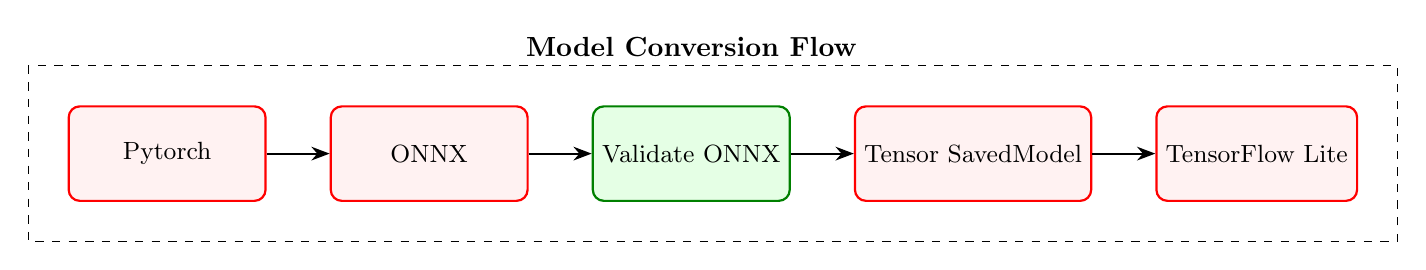
\begin{tikzpicture}[
    node distance=1cm and 0.8cm,
    box/.style={
      rectangle,
      rounded corners,
      minimum height=1.2cm,
      minimum width=2.5cm,
      fill=pink!20,
      draw=red,
      thick,
      align=center,
      font=\small
    },
    validate/.style={
      box,
      draw=green!50!black,
      fill=green!10
    },
    arrow/.style={
      -Stealth,
      thick
    }
  ]

  % Các node
  \node[box] (pytorch) {Pytorch};
  \node[box, right=of pytorch] (onnx) {ONNX};
  \node[validate, right=of onnx] (validate) {Validate ONNX};
  \node[box, right=of validate] (savedmodel) {Tensor SavedModel};
  \node[box, right=of savedmodel] (tflite) {TensorFlow Lite};

  % Các mũi tên
  \draw[arrow] (pytorch) -- (onnx);
  \draw[arrow] (onnx) -- (validate);
  \draw[arrow] (validate) -- (savedmodel);
  \draw[arrow] (savedmodel) -- (tflite);

  % Tiêu đề
  \node[above=0.5cm of validate, font=\bfseries] {Model Conversion Flow};

  % Viền ngoài
  \draw[dashed] ([xshift=-0.5cm, yshift=0.5cm]pytorch.north west) rectangle ([xshift=0.5cm, yshift=-0.5cm]tflite.south east);

  \end{tikzpicture}
  \caption{Model Conversion Flowchart}
  \label{fig:model_conversion_flow}
\end{figure}

% Ngăn các hình sau quay ngược lên trên
\FloatBarrier

Several libraries such as torch==2.3.0, onnx==1.16.2, onnx- are supported with model conversion process. tf==1.10.0, and tensorflow==2.14.0. Furthermore, the ONNX is also visually checkable with the Netron tool. It allows us to identify the potential issues with the input/output format before conversion, with the model architecture. This conversion takes place by converting the ONNX model into TensorFlow SavedModel format using default optimization settings and float32 precision. Then, the model is converted to TensorFlow Lite (TFLite). Explicitly avoiding to use FlexOps to not raise errors about unsupported operations like FlexS-SplitV. 
The following is the format of the input/output for the model after conversion:

\begin{itemize}
  \item \textbf{Input}: $[1, 640, 640, 3]$ --- which means a batch of one RGB image with spatial resolution $640\times640$.
  \item \textbf{Output}: $[1, 12, 8400]$ --- corresponding to the output predictions for each of the 8400 anchor points. The 12 predicted features per anchor include 4 bounding box coordinates (x, y, w, h) and 8 class scores \cite{yoloobjectfeatures}.
\end{itemize}

Some of the predicted features per anchor are 4 bounding box coordinates (x, y, w, h), 8 class scores \cite{18}.The set of features in earlier YOLO versions would usually include an objectness score that affected class predictions. During training it often suppressed loss of class which leads to degraded classification.
performance and dependence on anchor/grid design. For each pixel, the objectness and bounding was predicted. This leads to excessive redundant bounding boxes and strong post processing (e.g., Non Maximum
Suppression).


% Đảm bảo các hình trước đó không ảnh hưởng
\FloatBarrier

\begin{figure}[H] % Ép buộc vị trí tại đây
  \centering
  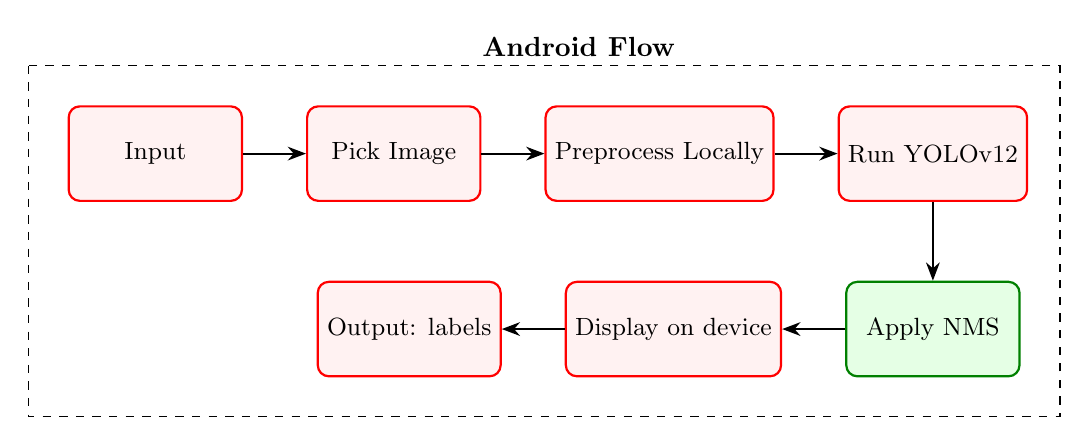
\begin{tikzpicture}[
    node distance=1cm and 0.8cm, % Khoảng cách giữa các node
    box/.style={
      rectangle,
      rounded corners,
      minimum height=1.2cm,
      minimum width=2.2cm, % Giữ chiều rộng vừa phải
      fill=pink!20,
      draw=red,
      thick,
      align=center,
      font=\small
    },
    nms/.style={
      box,
      draw=green!50!black,
      fill=green!10
    },
    arrow/.style={
      -Stealth,
      thick
    }
  ]

  % Các node - Hàng trên
  \node[box] (input) {Input};
  \node[box, right=of input] (pick) {Pick Image};
  \node[box, right=of pick] (preprocess) {Preprocess Locally};
  \node[box, right=of preprocess] (yolo) {Run YOLOv12};

  % Tính vị trí trung tâm của hàng trên
  \coordinate (center_top) at ($(input.west)!0.5!(yolo.east)$);

  % Hàng dưới - Căn giữa thủ công
  \node[nms, below=of yolo] (nms) {Apply NMS};
  \node[box, left=of nms] (display) {Display on device};
  \node[box, left=of display] (output) {Output: labels};

  % Điều chỉnh căn giữa hàng dưới
  \coordinate (center_bottom) at ($(output.west)!0.5!(nms.east)$);
  \path let \p1 = (center_top), \p2 = (center_bottom) in
    \pgfextra{\xdef\shiftamount{(\x1-\x2)}};
  \path (nms) [xshift=\shiftamount] (nms) (display) (output);

  % Các mũi tên
  \draw[arrow] (input) -- (pick);
  \draw[arrow] (pick) -- (preprocess);
  \draw[arrow] (preprocess) -- (yolo);
  \draw[arrow] (yolo) -- (nms); % Mũi tên đi xuống
  \draw[arrow] (nms) -- (display); % Mũi tên ngược lại sang trái
  \draw[arrow] (display) -- (output); % Mũi tên tiếp tục sang trái

  % Tiêu đề - Căn giữa
  \node[above=0.5cm of yolo, xshift=-4.5cm, font=\bfseries] {Android Flow};

  % Viền ngoài
  \draw[dashed] ([xshift=-0.5cm, yshift=0.5cm]input.north west) rectangle ([xshift=0.5cm, yshift=-0.5cm]nms.south east);

  \end{tikzpicture}
  \caption{Android Flowchart}
  \label{fig:android_flow}
\end{figure}

% Ngăn các hình sau quay ngược lên trên
\FloatBarrier


On the other hand, the objectness score is completely removed in YOLOv12. Rather than scanning the entire image with predefined anchors, the model uses queries: each of its query vector corresponds to a possible object. Without differentiating vectors associated with object or background, all 8400 vectors are treated as equal candidate vectors. In doing so, this paradigm shift eliminates the notion of a particular 'object center' in the image and simplifies model optimization while decreasing reliance on highly detailed anchor based heuristics.

All of the features are built on Flutter's widget system and implemented in separate screens. The application starts by running main.dart file, which initializes the application with MaterialApp and specifies routes to many screens including the home page, image selection, image capture, video selection, and real time recognition. Home\textunderscore screen.dart provides a welcome interface with navigation buttons that lead the user to each of the available functionality.

\begin{figure}[H]
  \centering
  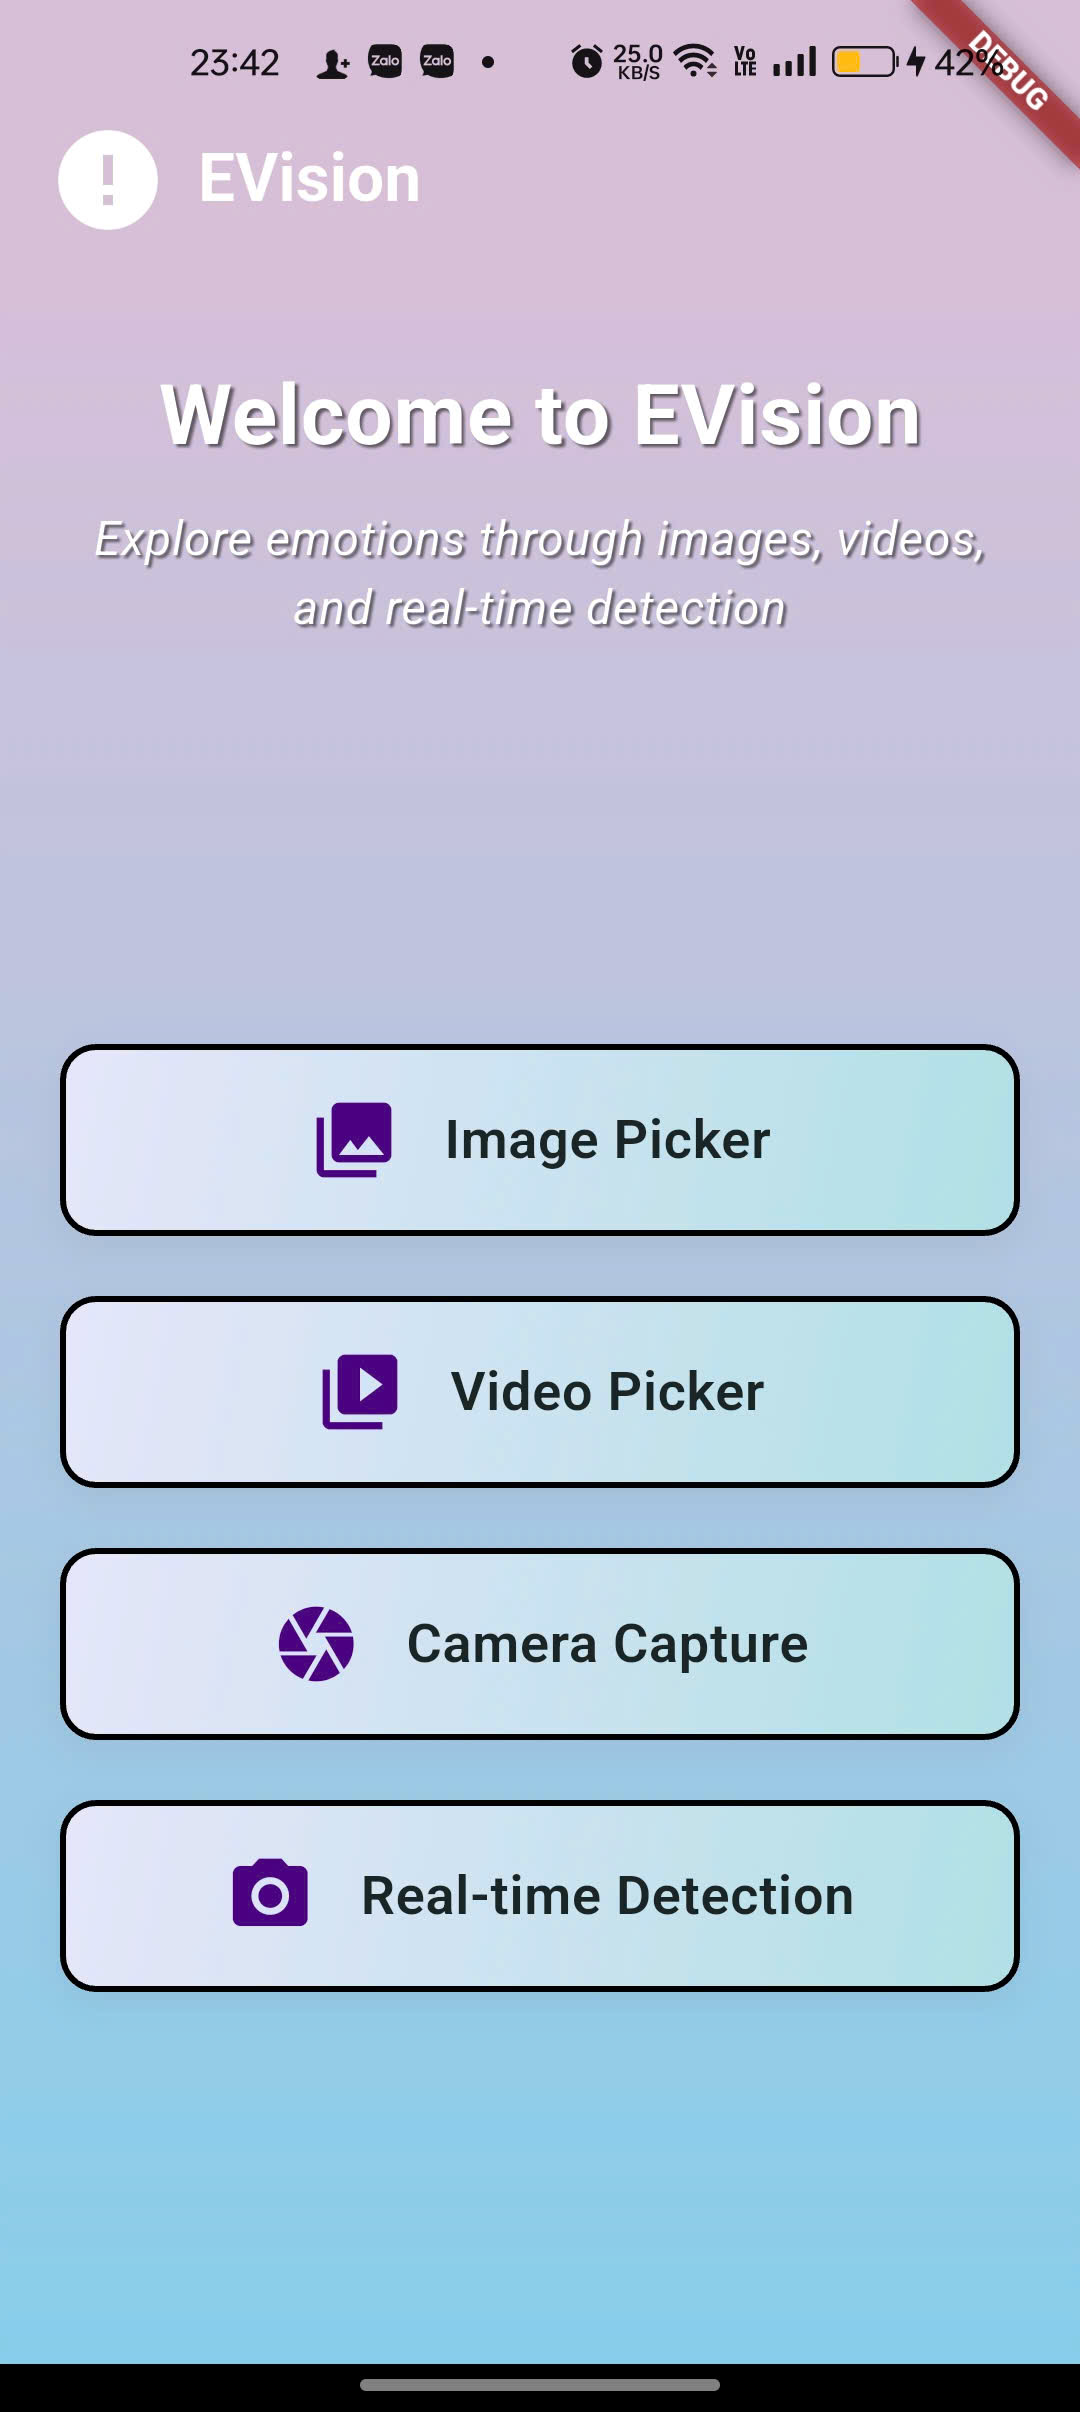
\includegraphics[scale=0.1]{homepage android.jpg}
  \caption{Android homepage display}
  \label{fig:method}
\end{figure}

The emotion detection functionality is the core of the ObjectDetector class, which is defined in object\textunderscore detector.dart. It loads the TensorFlow Lite model, as well as the labels.txt file that accompanies it from the assets directory. Moreover, we configure the model to run on 4 CPU threads for highest performance on mobile devices. Preprocessing input images includes resizing them to $640\times640$ pixels, padding with an additional 1 pixel border to get $642\times642$, and normalizing pixel values to $[0, 1]$ range.

The model takes an image tensor as input and outputs predictions (bounding boxes, emotion labels and confidence scores) via inference. Using the applyNMS function defined in utils.dart, the results are post processed by eliminating overlapping bounding boxes and keeping only the most accurate predictions.


Each feature screen integrates the ObjectDetector class in a distinct manner:
\begin{itemize}
  \item {Image Selection Screen}: With image\textunderscore picker package, users can select an image from gallery. It takes the selected image, converts it to bytes, decode it to get dimensions and run in a separate isolate to avoid UI lag. Bounding Box Painter is used to render detection results with bounding boxes, predicted emotions and their confidence scores in a list.

  \begin{figure}[H]
  \centering
  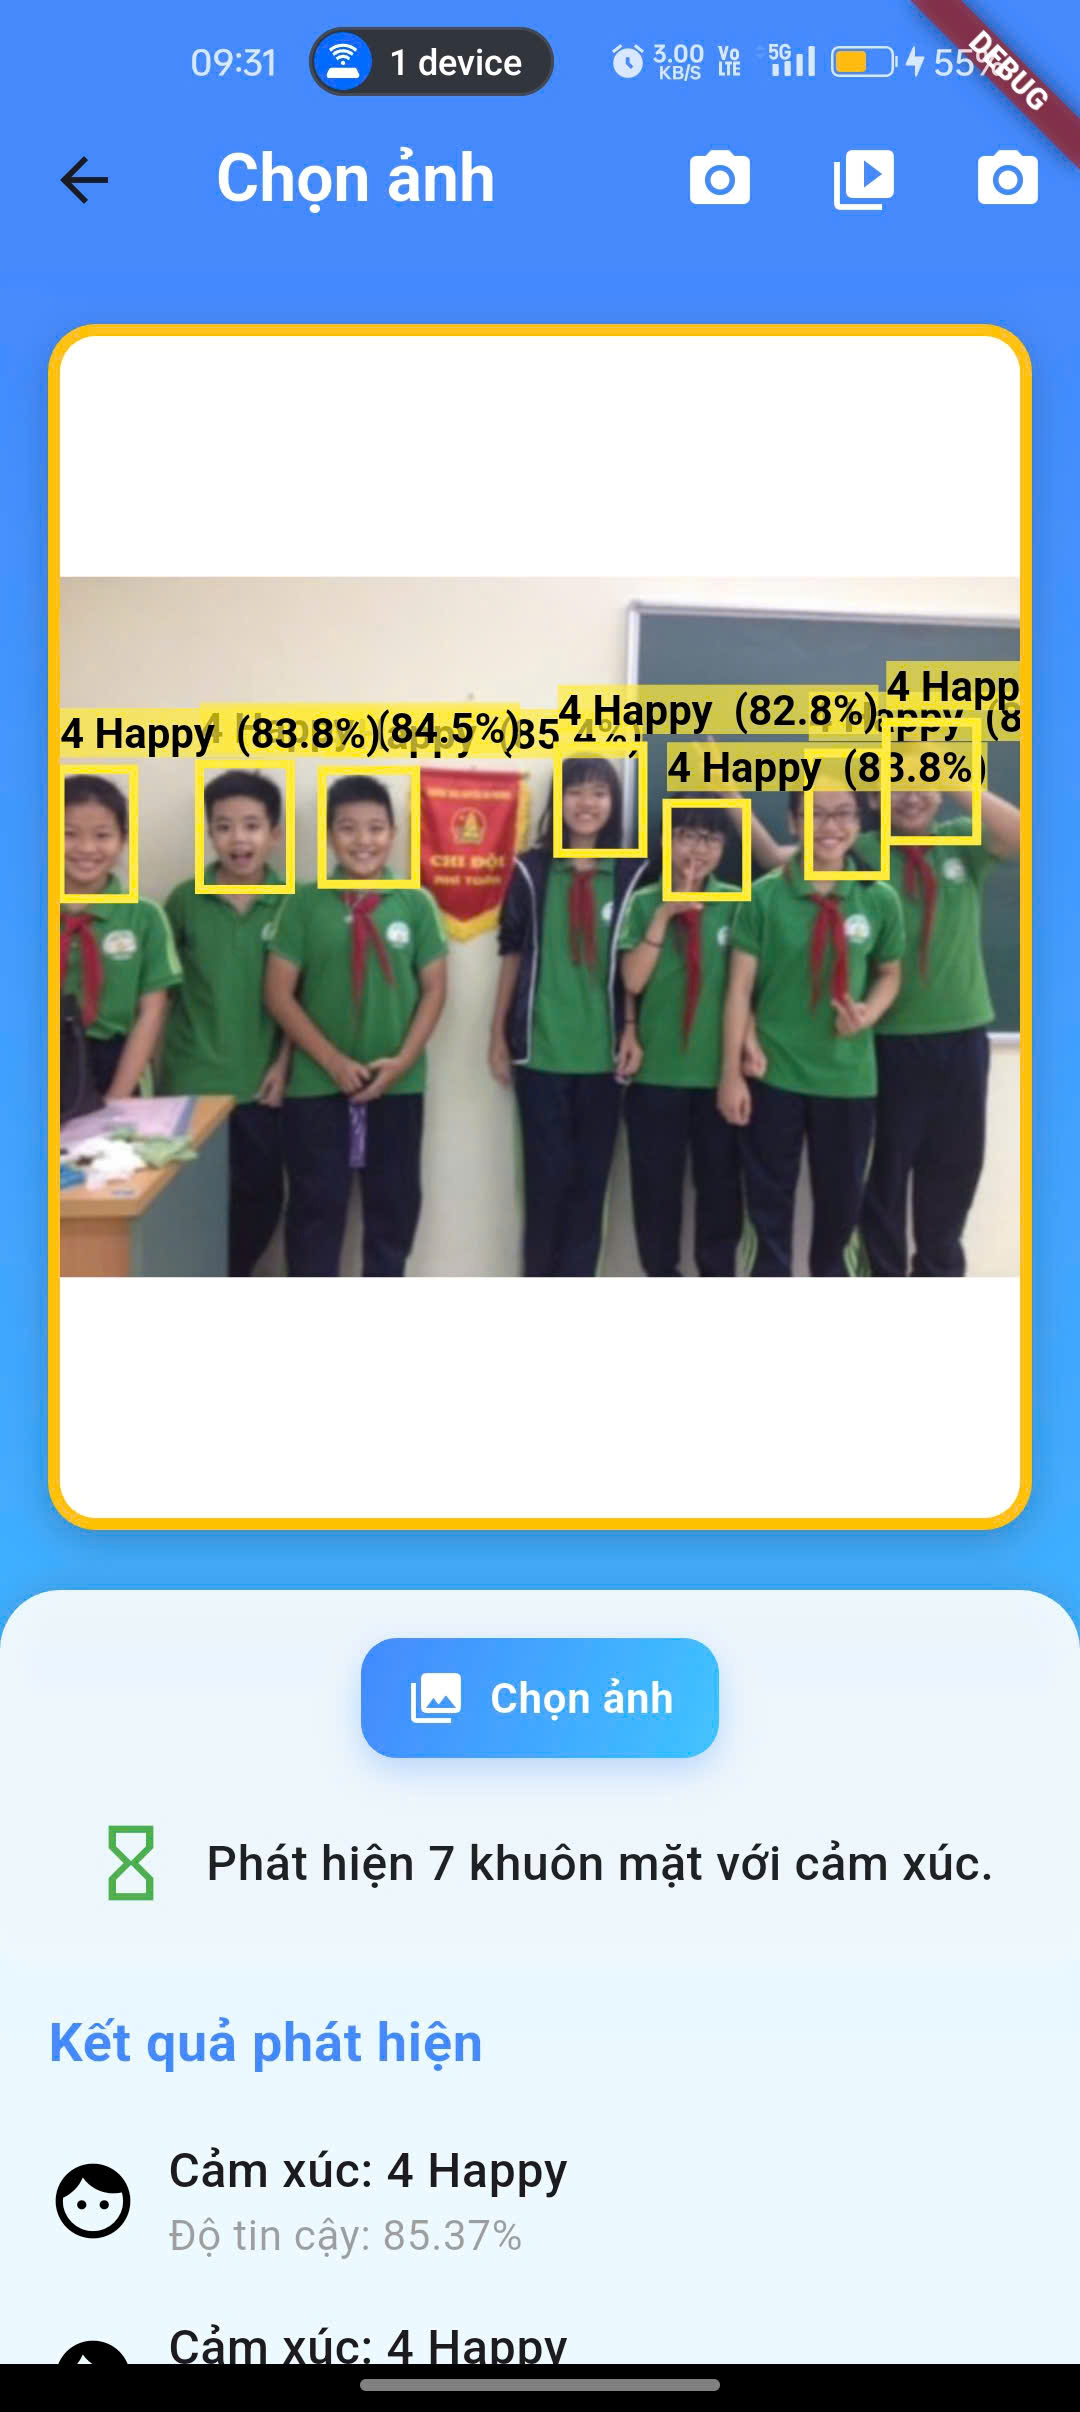
\includegraphics[scale=0.1]{image picker android.jpg}
  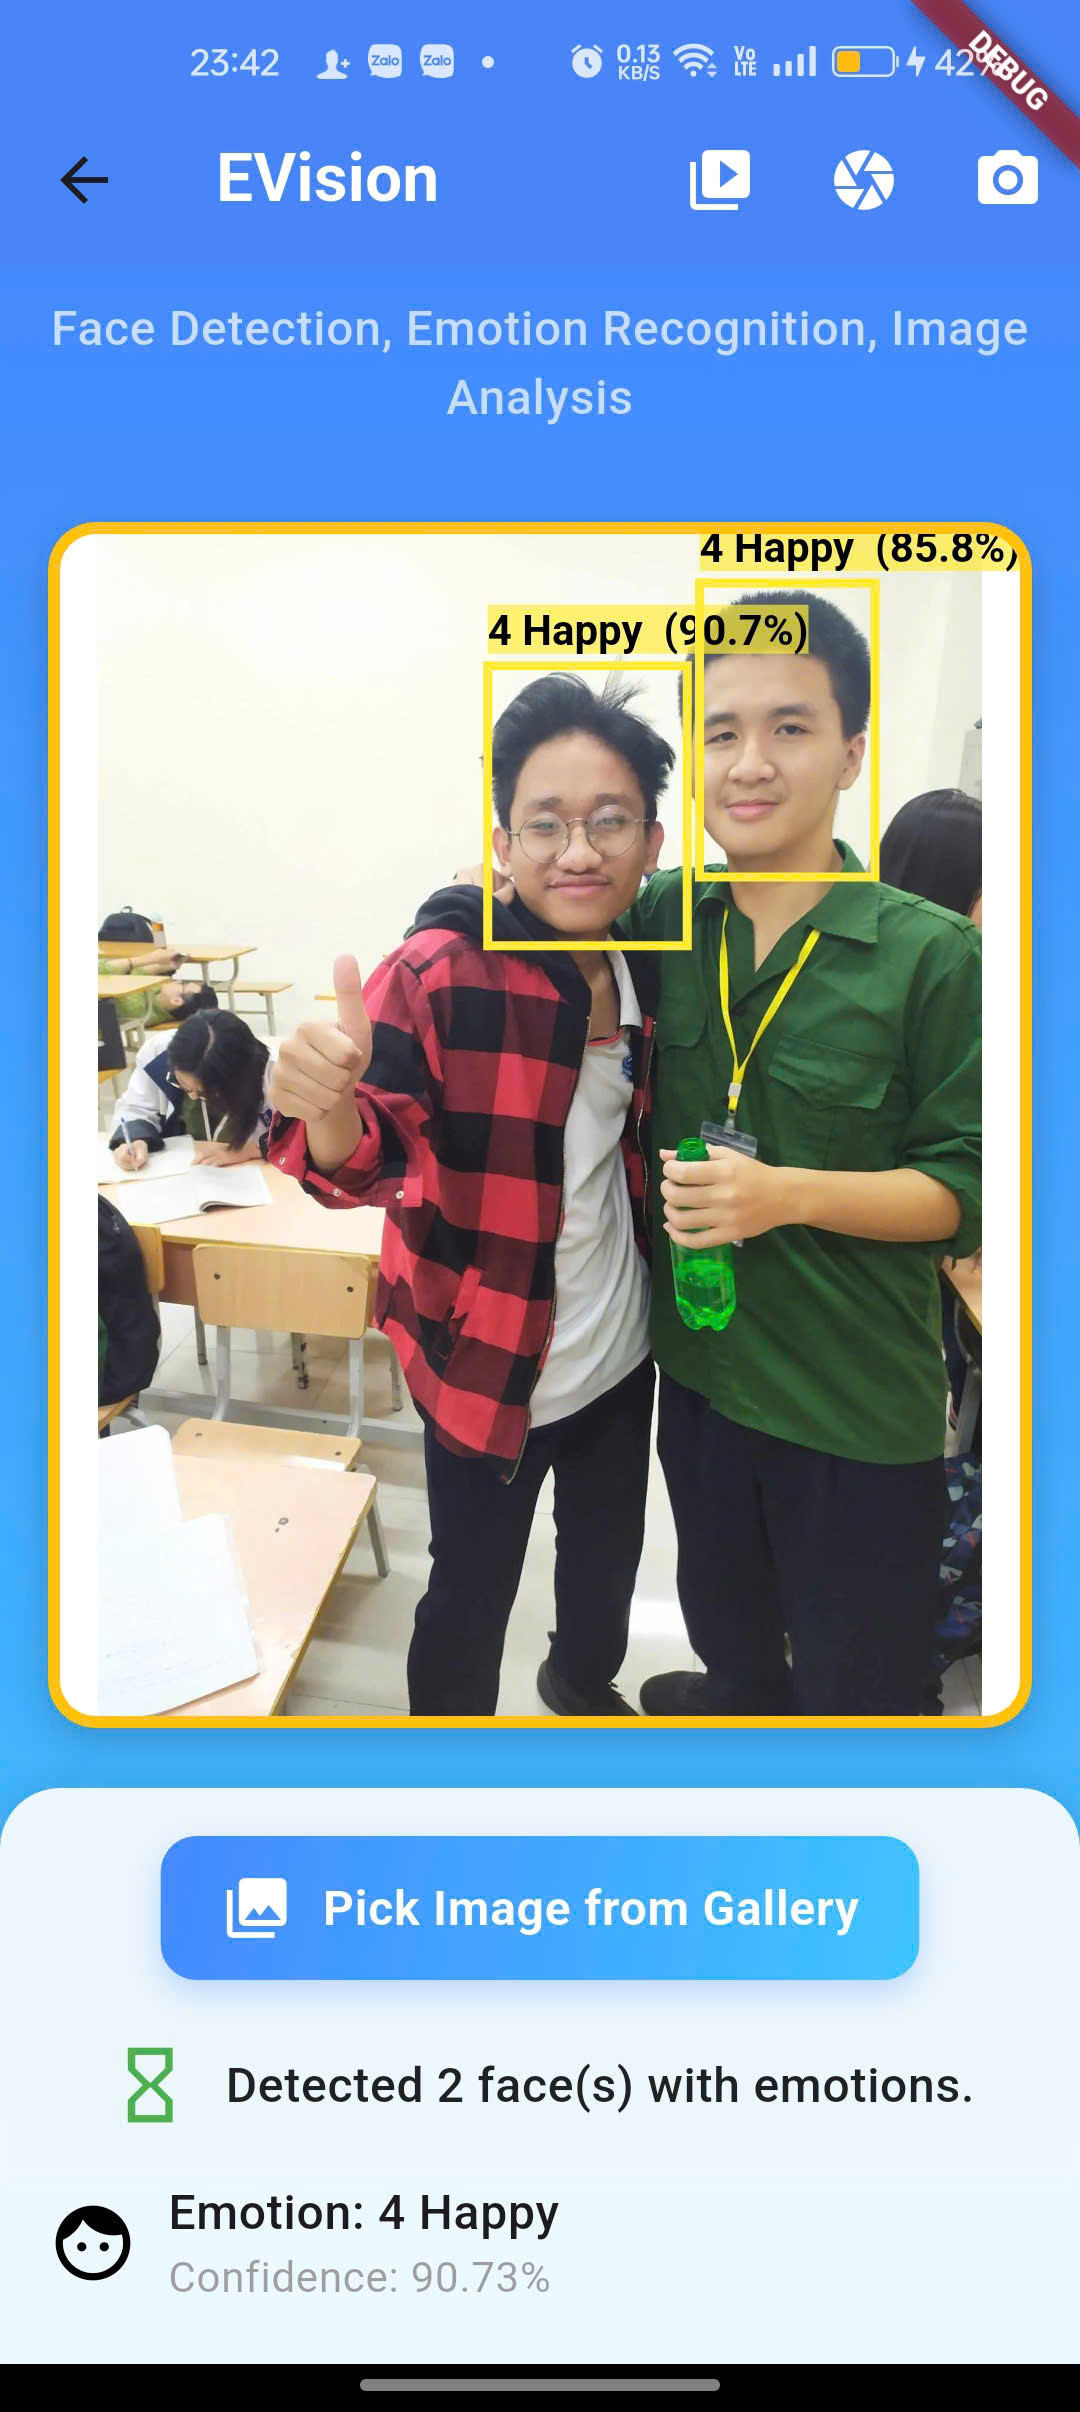
\includegraphics[scale=0.1]{image picker android 1.jpg}
  \includegraphics[scale=0.1]{image picker android 2.jpg}
  \caption{Android image picker function}
  \label{fig:method}
\end{figure}

.
  \item \textbf{Image Capture Screen}: It enables the users to capture a photo using the device camera. Results are displayed directly on the screen, and the same processing pipeline is applied to the captured image as to selected images.

  \begin{figure}[H]
  \centering
  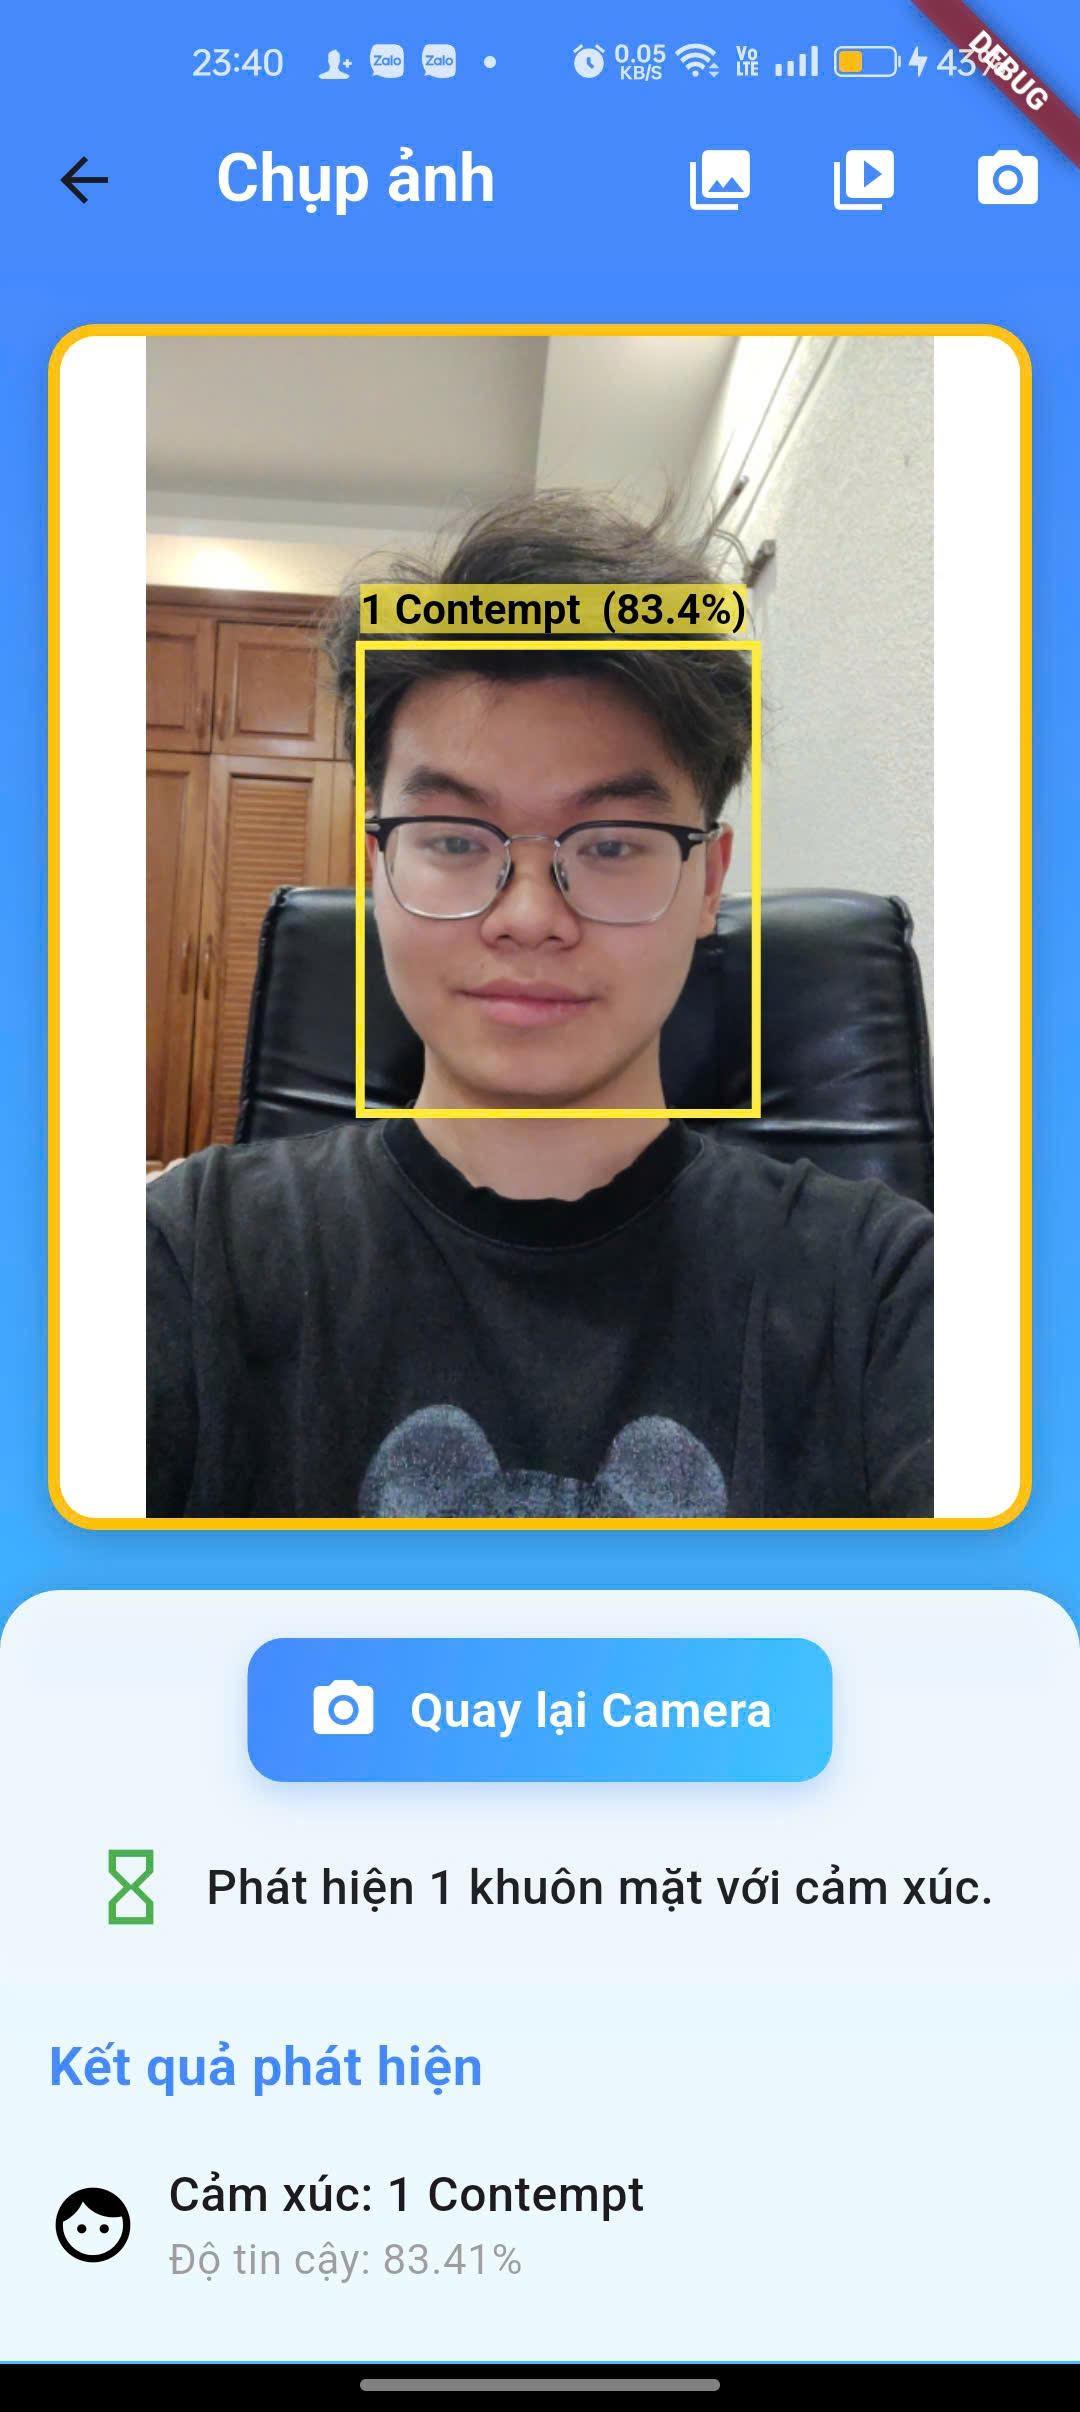
\includegraphics[scale=0.1]{camera capture android.jpg}
  \caption{Android camera capture function}
  \label{fig:method}
\end{figure}
  
  \item \textbf{Video Selection Screen}: The user can select a video from their device and take out the frames for emotion analysis. Results of detection are shown similarly, with video playback support to view analyzed content.
  \begin{figure}[H]
  \centering
  \includegraphics[scale=0.1]{video pick android.jpg}
  \caption{Android video picker function}
  \label{fig:method}
\end{figure}

  \item \textbf{Real-Time Detection Screen}: It uses the device camera to feed a live video stream and processes one frame every 500 milliseconds. The UI has bounding boxes and emotion labels going continuously and BoundingBoxPainter is used to draw on the live feed directly. This function however, we cannot develop it, but it will be developed in the future.

\end{itemize}

This also allows us to ensure that user interface always responds quickly, particularly in heavy tasks such as real time recognition, as we use isolates for inference. BoundingBoxPainter in bounding\textunderscore box\textunderscore painter.dart is used as a custom painter that draws bounding boxes and emotion labels on images and video frames with the colors and symbols for each emotion added to enhance visualization.

Finally, we are using the developer options on the phone’s settings, specifically USB Debugging, to install the built APK application on an actual phone instead of just running it on an emulator.

\section{Results achieved from the application}
We have successfully developed an application called ‘EVision’, which is a user friendly and comprehensive emotion recognition tool on two main platforms; web and Android.

The application has four main features available on the web platform: the image upload, webcam photo capture, video recording and real-time emotion recognition. The most striking is that we integrated an AI chatbot in real time mode that can respond in Vietnamese and then English intimately on detecting emotions, resulting in a great and effective experience. It uses pure javascript with flask so they can keep good performance and also have the aesthetics with gradient and shadow effects done in the web interface.
The application runs the emotion recognition model on the device using TensorFlow Lite, which helps improve performance on the device, reduce latency and keep it more secure. On the Android platform, the application is constructed using Flutter. Selection of images from the library, capturing from the camera, video analysis, real time recognition are some of the features and presented in a modern interface with a responsive design.
The application fulfilled its aim to become a solid sketch of a sentiment analysis application, which might go far in education, entertainment and mental health care. The use of Flutter also means that it is possible to expand to other platforms in the future.


% Chapter: Conclusion & Recommendations
\clearpage
\chapter{CONCLUSION \& RECOMMENDATIONS}
\section{Conclusion}
A brand new chatbot application called “Evision”, that can identify facial expressions in many different platforms, has been developed based on the YOLOv12 model, which able to detect and classify expression labels containing 7 emotional states. The key features such as using some images from the album, an web camera, analysing expressions in video and an emotional chat bot are integrated with Evoision. The Android platform can be built using the Flutter and TensorFlow Lite libraries for the best privacy of the users, whereas the web has the ability to interact with an AI chatbot based on real-time emotions.

The mAP@0.5 index achieved when running the system is 0.941 and the accuracy: 0.937 – recall: 0.989; a high level of accuracy in the field of emotion recognition. Evision not only contributes significantly to the intentional mechanism but also brings many practical meanings, especially in fields that require interaction.

\section{Recommendations}
\subsection{Limitation}
The Android version still lacks the AI chatbot, which has reduced user interaction and does not meet the comprehensiveness expected of a mobile application. Currently, the application is only being tested on Android devices, and the iOS version is still unavailable, resulting in a significant disadvantage for Apple users in accessing the application.

\subsection{Future development direction}
The application's accurate recognition interface needs to be further developed to improve the accuracy. The accuracy needs to be improved in difficult emotions and classification when the mask features are prone to duplication and cross-image anti-interference.

To reliably recognize high-level forms in different environments, developers need to address environmental factors such as lighting, image noise level when the camera scans, hidden face codes, etc. These factors can affect the system's ability to accurately recognize the interface.

In addition, we recommend integrating voice recognition or voice interaction microphone tools to enhance the application to allow users to communicate with AI naturally. The application user interface is adjusted to suit the voice features, microphone switch, real-time recording, ensuring a smooth and flexible user experience.

\newpage In fact, the extended application can meet the needs of users with entertainment features:

\begin{itemize}
  \item Automatically play videos or tips with the user's relaxation.
  \item Integrate API communications such as Twilio, Messenger to quickly connect with friends when detecting emotions swinging to too happy or too negative.
  \item AI-embedded chatbots are capable of chatting like humans using natural language processing techniques: DialogFlow, Rasa. Chatbots respond to emotional bases or store contextual content.
   \item Maximize flexibility by choosing different emotion recognition models based on the needs of the underlying device's performance capabilities.
\end{itemize}

Complex Vision Transformer models can increase performance at the highest accuracy. Add ccs option menu, language settings, tips.
To support mental health monitoring, the application can generate detailed reports on emotional trends over time. This includes visualizations such as weekly or monthly charts for the frequency and distribution of different emotional states, helping users track patterns and changes in their emotions.



% Chapter: References
\clearpage
\renewcommand{\bibname}{REFERENCE LIST}
\begin{thebibliography}{9}
\addcontentsline{toc}{section}{REFERENCE LIST}

\bibitem{ultralytics2025}
Ultralytics. (n.d.), \textit{YOLO12}, Retrieved April 14, 2025, from \textbf{https://docs.ultralytics.com/vi/models/yolo12}

\bibitem{bonsall2012}
Bonsall, M. B., Wallace-Hadrill, S. M., Geddes, J. R., Goodwin, G. M., \& Holmes, E. A. (2012), \textit{Nonlinear time-series approaches in characterizing mood stability and mood instability in bipolar disorder}, Proceedings of the Royal Society B: Biological Sciences, \textbf{279}(1730), 916–924.

\bibitem{guo2024}
Guo, R., Guo, H., Wang, L., Chen, M., Yang, D., \& Li, B. (2024), \textit{Development and application of emotion recognition technology—a systematic literature review}, BMC Psychology, \textbf{12}(1), 95. 

\bibitem{hale2021}
Hale, T., Angrist, N., Goldszmidt, R., Kira, B., Petherick, A., Phillips, T., Webster, S., Cameron-Blake, E., Hallas, L., \& Majumdar, S. (2021), \textit{A global panel database of pandemic policies (Oxford COVID-19 Government Response Tracker)}, Nature Human Behaviour, \textbf{5}(4), 529–538.

\bibitem{james1948}
James, W. (1948), \textit{What is emotion? 1884}.

\bibitem{lange2009}
Lange, C. G. (2009), \textit{The Emotions}, Cambridge Scholars Publishing.

\bibitem{oliver2020}
Oliver, N., Lepri, B., Sterly, H., Lambiotte, R., Deletaille, S., De Nadai, M., Letouzé, E., Salah, A. A., Benjamins, R., \& Cattuto, C. (2020), \textit{Mobile phone data for informing public health actions across the COVID-19 pandemic life cycle}, Science Advances, \textbf{6}, eabc0764.

\bibitem{alizadeh2017} Alizadeh, S., \& Fazel, A. (2017), \textit{Convolutional neural networks for facial expression recognition}, arXiv preprint, \textbf{arXiv:1704.06756}.

\bibitem{pellert2020}
Pellert, M., Schweighofer, S., \& Garcia, D. (2020), \textit{The individual dynamics of affective expression on social media}, EPJ Data Science, \textbf{9}(1), 1.

\bibitem{tian2025}
Tian, Y., Ye, Q., \& Doermann, D. (2025), \textit{Yolov12: Attention-centric real-time object detectors}, arXiv preprint arXiv:2502.12524. 

\bibitem{kaushik2017} Kaushik, M. S., \& Kandali, A. B. (2017), \textit{Recognition of facial expressions extracting salient features using local binary patterns and histogram of oriented gradients}, 2017 International Conference on Energy, Communication, Data Analytics and Soft Computing (ICECDS), \textbf{pp. 1201--1205}.

\bibitem{thang2020} 
Thang, N. C. (2020), \textit{Basics of Object Detection with R-CNN, Fast R-CNN, Faster R-CNN, and YOLO}, Mì AI, \textbf{https://miai.vn/2020/07/04/co-ban-ve-object-detection-voi-r-cnn-fast-r-cnn-faster-r-cnn-va-yolo/}.

\bibitem{redmon2016} Redmon, J., Divvala, S., Girshick, R., \& Farhadi, A. (2016), \textit{You only look once: Unified, real-time object detection}, Proceedings of the IEEE Conference on Computer Vision and Pattern Recognition, \textbf{pp. 779--788}.

\bibitem{yoloexplained} YOLO Object Detection Explained: A Beginner’s Guide, (n.d.), \textit{DataCamp}, \textbf{https://www.datacamp.com/blog/yolo-object-detection-explained}.

\bibitem{yolo2023} Understanding the YOLO Model from Past to Present, (2023), \textit{Exploring the World of AI Programming}, \textbf{https://tuhoclaptrinhsite.wordpress.com/2023/04/30/tim-hieu-mo-hinh-yolo-tu-qua-khu-toi-hien-tai/}.

\bibitem{roboflow2025} How to Train a YOLOv12 Object Detection Model on a Custom Dataset, (2025), \textit{Roboflow Blog}, \textbf{https://blog.roboflow.com/train-yolov12-model/}.

\bibitem{sharma2025} Sharma, B. (2025), \textit{YOLOv12: Object Detection Meets Attention}, LearnOpenCV, \textbf{https://learnopencv.com/yolov12/}.

\bibitem{yoloobjectfeatures} Retrieving Object-Level Features from YOLO, (n.d.), \textit{Y-T-G Tutorials}, \textbf{https://y-t-g.github.io/tutorials/yolo-object-features/}.


\end{thebibliography}

\end{document}